\section{Precomputing Binary Rank in Blocks}
During our experiment of skewing the tree, we concluded that most of the work during queries is performed inside each node, calculating the binary rank of each bitmap.
Rank queries are simply summing up results of popcounting each word, and we considered whether precomputing these sums for blocks spanning several words, covering the bitmaps could improve the query times.
When a block doesn't line up with the position a rank query is for, the algorithm can simply fall back to doing popcounting of either the remaining uncovered words or the excess covered words, whichever has fewer words.
See Section~\ref{sec:rankQueriesWithPrecomputedRanksEdgeCases} for more explanation of this.

We can precompute the rank values easily and cheaply by doing so as we build the tree where we already need to compute and store each individual bit of the bitmap.
We simply increment a counter for the corresponding block each time we set a bit to 1 in the bitmap.

The size of the precomputed blocks is a new variable that could have influence on the running time and memory usage.
Some advantages of larger blocks is less memory usage and fewer precomputed value lookups for the same part of the bitmap.
Some advantages of smaller blocks are that they can cover more precisely the part of the bitmap that is relevant to the query, leading to fewer calls to popcount.
We will experiment to find an optimal value for our system.

To further reduce the space used by the precomputed values, we considered concatenating all the bitmaps into one big bitmap as that would eliminate the many cases where the length of a bitmap doesn't align with the block size and the last precomputed value for that bitmap will therefore not cover an entire block, leading to more precomputed values than minimally needed to cover all the bitmaps.

We also considered the cost of TLB misses and how ensuring that entire pages are skipped as often as possible might increase the query performance. We try to achieve this by page-aligning the blocks.

We will test and compare the Rank and Select running times and memory usage of three wavelet trees using precomputed rank values for blocks: one using concatenated bitmaps and aligned blocks, one only using aligned blocks and one using neither.




\subsection{Concatenating the Bitmaps}
We allocate the bitmaps as one giant bitmap the size of the maximum possible size required to store all the bitmaps for all the nodes. The sum of the size of all bitmaps on one layer of the tree can at most be $n$ and we can at most have $h$ layers, so the maximum size becomes
\[n \cdot h\]
where $n$ is the number of characters in the string and $h$ is the max height of the binary wavelet tree which is
\[ h = log(\sigma) \]
Luckily for us, memory allocation in Linux doesn't actually take up space, only when it is accessed will the actual physical memory be used.
So over-allocating the bitmap should not take up any more space than will actually be needed.

We then store an offset and a size for the bitmap in each node, so we can index into the giant bitmap and access the bits corresponding to the node.
This should also cause an decrease in memory usage as the offset and size are stored in an unsigned long and unsigned int respectively, taking a total of $64+32=96$ bits per node, where each individual bitmap requires storage of at least a pointer to it, a point to where its internal array starts and a pointer to where it ends, taking up $3*64=192$ bits per node.
Additionally, when using an individual bitmap for each node, they would have been word-aligned, and the bits between the last used bit and the end of the last used word would have gone unused and so, wasted.

We also allocate a vector for holding the precomputed block values of size
\[ \frac{BitmapSize}{BlockSize} \]
Instead of storing a pointer to the bitmap and precomputed values vector in each node, we store them once for the whole tree and then pass them down through the query methods when the tree is queried.

We use integer division of the bitmap offset and the block size to index into said vector. It is an efficient and simple way to precompute the rank values of blocks of fixed size of the bitmap.


\subsubsection{Edge Cases}
\label{sec:rankQueriesWithPrecomputedRanksEdgeCases}
The rank of a string can be expressed as the sum of the rank of any number and various sizes of subparts as long as they together perfectly cover the string and don't overlap.
Because the blocks must perfectly cover the string and not overlap, and the bitmaps of each node are not of same size, nor multiples of some single value, we have a problem if we want to use uniformly sized and distributed blocks.
The problem exists at the boundary between bitmaps, where the precomputed rank value will be the sum of the rank of the end of the first bitmaps and the rank of the beginning of the second bitmap.

Looking at a single bitmap for a node, there is an edge case for the first and last part of the bitmap, because they don't fill an entire block, so we can't simply use the corresponding precomputed value as-is.
Instead, we can compute the rank of the part of the block that our part doesn't fill and subtract that from the precomputed rank value.
This is only worth doing when our part fills more than half a block, because then the other part is smaller than half a block and therefore quicker to compute.
Figure ~\ref{fig:PrecomputePopcountBlock} illustrates this.



\figureBegin
\caption{Rank value of a part of a bitmap is equal to the precomputed value for the block minus the rank of the other remaining part.}
\label{fig:PrecomputePopcountBlock}
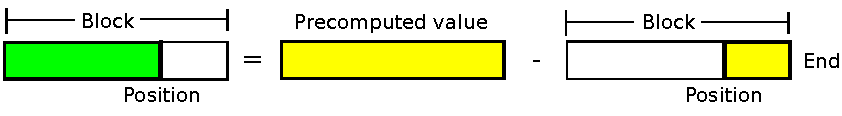
\includegraphics[width=\textwidth]{PrecomputePopcountBlock.pdf}
\figureEnd




%\begin{algorithm}
%\caption{Rank Query for PreallocatedPrecomputed}
%\label{dsfdsfsd}
%\begin{algorithmic}
%\State \Comment{\textproc{PopcountRank} is a function that calculates the rank of a given part of a bitmap using the popcount cpu instruction}
%\Function{Rank}{Position, Bitmap, PrecomputedRanks}
%\If{Position $<$ BlockSize/2}
%\State \Return \Call{PopcountRank}{This bitmap}
%\EndIf
%\If{Position $<$ BlockSize \textit{and} Position $<$ LengthToNextBlock}
%\State PreRank $\gets$ \Call{PopcountRank}{Part of block before this bitmap}
%\State PostRank $\gets$ \Call{PopcountRank}{Part of block after this bitmap}
%\State BlockIndex $\gets$ \textit{Index of the block this bitmap is in}
%\State \Return PrecomputedRanks[BlockIndex] - PreRank - PostRank
%\EndIf
%\If{
%\EndFunction
%\end{algorithmic}
%\end{algorithm}




\subsubsection{Page-aligning the Blocks}
Translation Lookaside Buffer misses are expensive and to avoid those, we can try to reduce the number of pages we load.
Using concatenated bitmaps and the precomputed vector of ranks, we only need to load pages of the bitmap at the beginning and end of each node's bitmap, to compute the popcount binary rank directly on the bitmap, and only within one block at each end.
If the blocks are not aligned with the memory pages, then, even if the block size is less than a page, it might span more than one page and thus more than one page of memory must be loaded into the TLB.
More precisely, we might at most load $2 \cdot \left( \lceil\frac{blockSize}{pageSize}\rceil +1 \right)$ pages to do the popcount binary rank computation at the beginning and end of each node.

If we page-align the blocks, and use block sizes divisible by the page size or that the page is divisible by, the extra $+1$ will disappear, because a block can no longer span more pages than its size is a multiple of the page size.
This means we can ensure that at most $2 \cdot \lceil\frac{blockSize}{pageSize}\rceil$ memory pages of the bitmap are loaded for each node by page-aligning the blocks.
With an alphabet size of $2^{16}$ this amounts to saving up to 16 page loads per query.

While we expect that this will save some expensive TLB misses it also has some drawbacks, especially when not using concatenated bitmaps.
For a wavelet tree not using concatenated bitmaps, using page-aligned blocks will cause the first precomputed value of each non-page-aligned bitmap to not cover an entire block, increasing the number of precomputed values needed to cover the bitmap as well as additional computations to calculate exactly which part of the bitmap it covers.
For the wavelet trees using concatenated bitmaps, these computations are needed regardless of block alignment, as the blocks are already not aligned with the individual bitmaps, and so we believe it can only be an improvement to page-align the blocks in this case. \textbf{[TODO: should we test this anyway?]}

We will test whether it increases the performance of rank and select queries when not using concatenated bitmaps in section~\ref{sec:queryRunTimePrecomputedBlockSizes}.


\subsection{Select Queries with Precomputed Ranks}
Select queries, although they don't return a rank value, can still utilize the precomputed rank values to skip much computation directly on the bitmap by iterating though them.
Partway in a select query, if the sum of the occurrences found so far and the rank value of the current block of the bitmap is more than the queried-for occurrence, we can add that rank value to our occurrences seen so far and skip ahead to the next block and perform the same test.
If the sum is less than the queried-for occurrence, we know we will find the occurrence in the current block and use our previously implemented method of calculating select using popcount, starting at this block.


\subsubsection{Edge Cases}
As with rank queries, there are edge cases at the beginning and end of each bitmap.
However, in this case, the edge case at the end is easily handled as the test of sum of rank and occurrence-so-far should fail, sending the algorithm into the block with the previous select query method, finding the occurrence with no problem and no specific handling of the edge case.
This is assuming the input occurrence parameter is valid, that is, at least that many occurrences of that character is in the original input string.

For the other case, at the beginning of the bitmap, we do almost exactly the same as in the case for the rank query.
In fact, we use a rank query to calculate the rank of the first part of the bitmap, using the trick of subtracting from the precomputed value if larger than half a block size, to figure out whether the occurrence is in the first part of the bitmap, and therefore whether we should skip it or not.

\paragraph{Using Rank Queries in Select Queries}~\\
We would like to analyse whether it is worth using a rank query to find out whether we should do a select query on the first part of the bitmap, as the rank query is purely extra work in the cases where the occurrence is in that part of the bitmap.

We will assume an equal number of occurrences in the string of each character in the alphabet, a uniform distribution of each character in the string, and an equal probability of each valid parameter for the select query.
A valid character parameter is one that exists in the input string and a valid occurrence parameter is an integer above 0 and below or equal to the number occurrences appearing in the input string.

The rank query is a computation of worst-case cost $\frac{blockSize}{2}$ because it will at most popcount half of the block, because we utilize the precomputed rank value when advantageous.
The popcount select query into the first partial block is an operation of word-case cost $blockSize$ because it can at most popcount the entire block.
So, in the worst case, when the sought-after occurrence is in the first partial block of the bitmap, $\frac{blockSize}{2}$ work is wasted, yet when the occurrence is elsewhere, $blockSize$ work is saved.
This means that the boundary between where using the rank query becomes a gain or a loss in performance is where the ratio between times the occurrence is to be found in and outside the first partial block of the bitmap is $\nicefrac{2}{3}$.
That is, when the occurrence is to be found outside the first partial block of the bitmap less than two-thirds of the time, using the rank query first to see if that partial block should be select queried is a gain in performance, when considering the worst-case query time for both queries.

Though, this is giving the select query a disadvantage in the analysis, as, even when the partial block is close to a block in size, it might terminate early if it found the sought-after occurrence of the character early in the partial block.

It is not entirely clear whether it is an advantage to use the binary rank call, or it would be better to use popcount BinarySelect on the first partial block at all times.
We will test this in section~\ref{sec:experimentPrecomputedBlocksRankInSelect}
\textbf{[TODO]}



\subsection{Extra Space Used by Precomputed Values}
Since each precomputed value cannot exceed the block size in bits, assuming we don't use block sizes exceeding $2^{16} = 65536$ bits, or $\frac{2^{16}}{8} = 8192$ bytes, we can store them in 16-bit unsigned integers, called \texttt{unsigned short int} in C++ on our machines.
Since the page size on our machines are 4096 bytes we should not use a block size larger than $\frac{8192}{4096} = 2$ pages if we want to use 16-bit unsigned integers.

In Section~\ref{sec:queryRunTimePrecomputedBlockSizes} we find that the optimal block size is 16384 bits = 2048 bytes = $\nicefrac{1}{2}$ page.

Assuming we then store the precomputed values as 16-bit unsigned short integers it will only consume an extra 16 bits or 2 bytes per block of which there are $\frac{BitmapSize}{BlockSize}$ when we concatenate the bitmaps.
This means, assuming a block size of 2048 bytes, a relative extra space consumption of
\[ \frac{ 2 \cdot \frac{BitmapSize}{BlockSize} }{BitmapSize} = \frac{2}{BlockSize} = \frac{2}{2048} = 0.0009765625 = 0.098\% \]
of the bitmaps.
Which is even less when considering the total space used including the nodes.

When we don't concatenate the bitmaps there is a higher space consumption by the precomputed values, as each precomputed value don't cover an entire block and more precomputed values is therefore needed to cover all the bitmaps.
When the blocks are not page-aligned, each node has potentially one precomputed value not covering an entire block at the end of its bitmap.
When blocks are page-aligned, there is another precomputed value potentially not covering an entire block at the beginning of each bitmap.
The extra space consumption by the precomputed values when not concatenating the bitmaps is therefore limited proportionally to the number of nodes, which is at most $2 \sigma - 1$, making it limited proportionally by the alphabet size.

We expect to see a difference in memory usage between using concatenated bitmaps and non-concatenated bitmaps as well as between using page-aligned and non-page-aligned blocks.
However, we expect most of the difference to come from the space used by the bitmaps themselves, and therefore a noticeable difference between the data structure concatenating the bitmaps and the others, with a little difference between using page-aligned and non-page-aligned blocks, with the one using page-aligned blocks using most memory.



\subsection{Experiments}
We will test and compare the Rank and Select running times of three wavelet trees using precomputed rank values for varying block sizes: one using concatenated bitmaps and aligned blocks named PreallocatedPrecomputed, one using aligned blocks but not concatenated bitmaps, called NaivePrecomputed,
and one using unaligned blocks and non-concatenated bitmaps called UnalignedNaivePrecomputed.
In table-form:\\
\begin{tabular}{|l|c|c|}
\hline
Name							& Concat. Bitmaps	& Page-aligned Blocks	\\ \hline
PreallocatedPrecomputed		& yes				& yes					\\ \hline
NaivePrecomputed				& no					& yes					\\ \hline
UnalignedNaivePrecomputed	& no					& no						\\ \hline
\end{tabular}

Later, we will compare the memory usage and query times with the non-precomputed version, called NaiveInteger.

\subsubsection{Query Running Time for Bitmap with Precomputed Blocks for different Block Sizes}
\label{sec:queryRunTimePrecomputedBlockSizes}

\paragraph{Rank Queries}~\\
In Figure~\ref{fig:PrecomputedRankBlockSize_Rank_WallTime} we have plotted the rank query wall time in $\mu s$ for the wavelet trees using precomputed rank values.

We see that PreallocatedPrecomputed is consistently slower than the other two, as expected, taking about ??\% more time than UnalignedNaivePrecomputed with block size = 0.5 page where Unaligned is fastest, and ??\% more with block size = 1 page where Preallocated is fastest.

Much of the increased running time of Rank queries on the PreallocatedPrecomputed wavelet tree can likely be explained by the increased amount of instructions needed to calculate the rank of the first part inside the first block of each bitmap because the precomputed value includes part of the preceding bitmap, as well as the ineffectiveness of utilizing the precomputed rank values for small bitmaps, for the same reason.
However, by examining Figure~\ref{fig:PrecomputedRankBlockSize_Rank_BranchMiss} and \ref{fig:PrecomputedRankBlockSize_Rank_BranchMissRate} we can conclude that part of the increase, at least in comparison with NaiveInteger, is also due to the increased number of branch misses.

In Figure~\ref{fig:PrecomputedRankBlockSize_Rank_BranchMissRate} we also see a surprising increase in the branch misprediction rate of UnalignedNaivePrecomputed for smaller block sizes.
When looking at Figure~\ref{fig:PrecomputedRankBlockSize_Rank_BranchMiss} we see that it follows the same increase in amount for smaller block sizes as the others, making us conclude that UnalignedNaivePrecomputed must simply run less branching code than the others for smaller block sizes.
This is likely simply a result of UnalignedNaivePrecomputed not having to do any calculations to figure out what part of the bitmap the first precomputed value covers, as it always covers an entire block of the bitmap.

Looking at Figure~\ref{fig:PrecomputedRankBlockSize_Rank_TLB} we can see that our expressed goal of reducing TLB misses is achieved when both concatenated bitmaps and page-aligned blocks are used. \textbf{[TODO: we should probably implement and test a concat.-bitmap-using non-page-aligned-blocks tree]}




We can also see that page-aligning the blocks when not using concatenated bitmaps is not an improvement in regards to rank query wall time.
In Figure~\ref{fig:PrecomputedRankBlockSize_Rank_TLB} we can however see that it actually does reduce TLB misses compared to the unaligned case, as was the intention of the modification, but only by about 4,45\% at block size = 0.5 page size which is even within the average relative standard deviation of both NaivePrecomputed and UnalignedNaivePrecomputed, making it close to pointless.



\figureBegin
\caption{Wall Time of Rank queries on wavelet trees with precomputed ranks of varying block sizes}
\label{fig:PrecomputedRankBlockSize_Rank_WallTime}
% GNUPLOT: LaTeX picture with Postscript
\begingroup
  \makeatletter
  \providecommand\color[2][]{%
    \GenericError{(gnuplot) \space\space\space\@spaces}{%
      Package color not loaded in conjunction with
      terminal option `colourtext'%
    }{See the gnuplot documentation for explanation.%
    }{Either use 'blacktext' in gnuplot or load the package
      color.sty in LaTeX.}%
    \renewcommand\color[2][]{}%
  }%
  \providecommand\includegraphics[2][]{%
    \GenericError{(gnuplot) \space\space\space\@spaces}{%
      Package graphicx or graphics not loaded%
    }{See the gnuplot documentation for explanation.%
    }{The gnuplot epslatex terminal needs graphicx.sty or graphics.sty.}%
    \renewcommand\includegraphics[2][]{}%
  }%
  \providecommand\rotatebox[2]{#2}%
  \@ifundefined{ifGPcolor}{%
    \newif\ifGPcolor
    \GPcolortrue
  }{}%
  \@ifundefined{ifGPblacktext}{%
    \newif\ifGPblacktext
    \GPblacktexttrue
  }{}%
  % define a \g@addto@macro without @ in the name:
  \let\gplgaddtomacro\g@addto@macro
  % define empty templates for all commands taking text:
  \gdef\gplbacktext{}%
  \gdef\gplfronttext{}%
  \makeatother
  \ifGPblacktext
    % no textcolor at all
    \def\colorrgb#1{}%
    \def\colorgray#1{}%
  \else
    % gray or color?
    \ifGPcolor
      \def\colorrgb#1{\color[rgb]{#1}}%
      \def\colorgray#1{\color[gray]{#1}}%
      \expandafter\def\csname LTw\endcsname{\color{white}}%
      \expandafter\def\csname LTb\endcsname{\color{black}}%
      \expandafter\def\csname LTa\endcsname{\color{black}}%
      \expandafter\def\csname LT0\endcsname{\color[rgb]{1,0,0}}%
      \expandafter\def\csname LT1\endcsname{\color[rgb]{0,1,0}}%
      \expandafter\def\csname LT2\endcsname{\color[rgb]{0,0,1}}%
      \expandafter\def\csname LT3\endcsname{\color[rgb]{1,0,1}}%
      \expandafter\def\csname LT4\endcsname{\color[rgb]{0,1,1}}%
      \expandafter\def\csname LT5\endcsname{\color[rgb]{1,1,0}}%
      \expandafter\def\csname LT6\endcsname{\color[rgb]{0,0,0}}%
      \expandafter\def\csname LT7\endcsname{\color[rgb]{1,0.3,0}}%
      \expandafter\def\csname LT8\endcsname{\color[rgb]{0.5,0.5,0.5}}%
    \else
      % gray
      \def\colorrgb#1{\color{black}}%
      \def\colorgray#1{\color[gray]{#1}}%
      \expandafter\def\csname LTw\endcsname{\color{white}}%
      \expandafter\def\csname LTb\endcsname{\color{black}}%
      \expandafter\def\csname LTa\endcsname{\color{black}}%
      \expandafter\def\csname LT0\endcsname{\color{black}}%
      \expandafter\def\csname LT1\endcsname{\color{black}}%
      \expandafter\def\csname LT2\endcsname{\color{black}}%
      \expandafter\def\csname LT3\endcsname{\color{black}}%
      \expandafter\def\csname LT4\endcsname{\color{black}}%
      \expandafter\def\csname LT5\endcsname{\color{black}}%
      \expandafter\def\csname LT6\endcsname{\color{black}}%
      \expandafter\def\csname LT7\endcsname{\color{black}}%
      \expandafter\def\csname LT8\endcsname{\color{black}}%
    \fi
  \fi
  \setlength{\unitlength}{0.0500bp}%
  \begin{picture}(7488.00,4464.00)%
    \gplgaddtomacro\gplbacktext{%
      \csname LTb\endcsname%
      \put(1210,704){\makebox(0,0)[r]{\strut{} 0}}%
      \put(1210,948){\makebox(0,0)[r]{\strut{} 2000}}%
      \put(1210,1193){\makebox(0,0)[r]{\strut{} 4000}}%
      \put(1210,1437){\makebox(0,0)[r]{\strut{} 6000}}%
      \put(1210,1682){\makebox(0,0)[r]{\strut{} 8000}}%
      \put(1210,1926){\makebox(0,0)[r]{\strut{} 10000}}%
      \put(1210,2170){\makebox(0,0)[r]{\strut{} 12000}}%
      \put(1210,2415){\makebox(0,0)[r]{\strut{} 14000}}%
      \put(1210,2659){\makebox(0,0)[r]{\strut{} 16000}}%
      \put(1342,484){\makebox(0,0){\strut{} 0}}%
      \put(1917,484){\makebox(0,0){\strut{} 20000}}%
      \put(2492,484){\makebox(0,0){\strut{} 40000}}%
      \put(3067,484){\makebox(0,0){\strut{} 60000}}%
      \put(3642,484){\makebox(0,0){\strut{} 80000}}%
      \put(4217,484){\makebox(0,0){\strut{} 100000}}%
      \put(4791,484){\makebox(0,0){\strut{} 120000}}%
      \put(5366,484){\makebox(0,0){\strut{} 140000}}%
      \put(5941,484){\makebox(0,0){\strut{} 160000}}%
      \put(6516,484){\makebox(0,0){\strut{} 180000}}%
      \put(7091,484){\makebox(0,0){\strut{} 200000}}%
      \put(176,1681){\rotatebox{-270}{\makebox(0,0){\strut{}Wall Time}}}%
      \put(4216,154){\makebox(0,0){\strut{}Block Size in bits}}%
    }%
    \gplgaddtomacro\gplfronttext{%
      \csname LTb\endcsname%
      \put(6600,4181){\makebox(0,0)[r]{\strut{}NaivePrecomputed, $mr\hat{\sigma}= $0.63 $avg\hat{\sigma}= $1.297}}%
      \csname LTb\endcsname%
      \put(6600,3741){\makebox(0,0)[r]{\strut{}PreallocatedPrecomputed, $mr\hat{\sigma}= $3.33 $avg\hat{\sigma}= $11.794}}%
      \csname LTb\endcsname%
      \put(6600,3301){\makebox(0,0)[r]{\strut{}UnalignedNaivePrecomputed, $mr\hat{\sigma}= $0.69 $avg\hat{\sigma}= $1.875}}%
    }%
    \gplbacktext
    \put(0,0){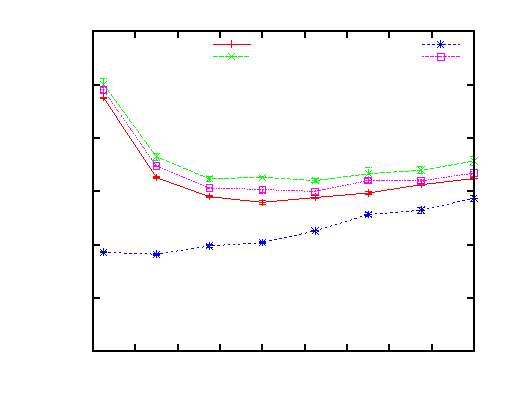
\includegraphics{PrecomputedRankBlockSize_Rank_WallTime}}%
    \gplfronttext
  \end{picture}%
\endgroup

\figureEnd


\figureBegin
\caption{Total Cycles of Rank queries on wavelet trees with precomputed ranks of varying block sizes}
\label{fig:PrecomputedRankBlockSize_Rank_TotalCycles}
% GNUPLOT: LaTeX picture with Postscript
\begingroup
  \makeatletter
  \providecommand\color[2][]{%
    \GenericError{(gnuplot) \space\space\space\@spaces}{%
      Package color not loaded in conjunction with
      terminal option `colourtext'%
    }{See the gnuplot documentation for explanation.%
    }{Either use 'blacktext' in gnuplot or load the package
      color.sty in LaTeX.}%
    \renewcommand\color[2][]{}%
  }%
  \providecommand\includegraphics[2][]{%
    \GenericError{(gnuplot) \space\space\space\@spaces}{%
      Package graphicx or graphics not loaded%
    }{See the gnuplot documentation for explanation.%
    }{The gnuplot epslatex terminal needs graphicx.sty or graphics.sty.}%
    \renewcommand\includegraphics[2][]{}%
  }%
  \providecommand\rotatebox[2]{#2}%
  \@ifundefined{ifGPcolor}{%
    \newif\ifGPcolor
    \GPcolortrue
  }{}%
  \@ifundefined{ifGPblacktext}{%
    \newif\ifGPblacktext
    \GPblacktexttrue
  }{}%
  % define a \g@addto@macro without @ in the name:
  \let\gplgaddtomacro\g@addto@macro
  % define empty templates for all commands taking text:
  \gdef\gplbacktext{}%
  \gdef\gplfronttext{}%
  \makeatother
  \ifGPblacktext
    % no textcolor at all
    \def\colorrgb#1{}%
    \def\colorgray#1{}%
  \else
    % gray or color?
    \ifGPcolor
      \def\colorrgb#1{\color[rgb]{#1}}%
      \def\colorgray#1{\color[gray]{#1}}%
      \expandafter\def\csname LTw\endcsname{\color{white}}%
      \expandafter\def\csname LTb\endcsname{\color{black}}%
      \expandafter\def\csname LTa\endcsname{\color{black}}%
      \expandafter\def\csname LT0\endcsname{\color[rgb]{1,0,0}}%
      \expandafter\def\csname LT1\endcsname{\color[rgb]{0,1,0}}%
      \expandafter\def\csname LT2\endcsname{\color[rgb]{0,0,1}}%
      \expandafter\def\csname LT3\endcsname{\color[rgb]{1,0,1}}%
      \expandafter\def\csname LT4\endcsname{\color[rgb]{0,1,1}}%
      \expandafter\def\csname LT5\endcsname{\color[rgb]{1,1,0}}%
      \expandafter\def\csname LT6\endcsname{\color[rgb]{0,0,0}}%
      \expandafter\def\csname LT7\endcsname{\color[rgb]{1,0.3,0}}%
      \expandafter\def\csname LT8\endcsname{\color[rgb]{0.5,0.5,0.5}}%
    \else
      % gray
      \def\colorrgb#1{\color{black}}%
      \def\colorgray#1{\color[gray]{#1}}%
      \expandafter\def\csname LTw\endcsname{\color{white}}%
      \expandafter\def\csname LTb\endcsname{\color{black}}%
      \expandafter\def\csname LTa\endcsname{\color{black}}%
      \expandafter\def\csname LT0\endcsname{\color{black}}%
      \expandafter\def\csname LT1\endcsname{\color{black}}%
      \expandafter\def\csname LT2\endcsname{\color{black}}%
      \expandafter\def\csname LT3\endcsname{\color{black}}%
      \expandafter\def\csname LT4\endcsname{\color{black}}%
      \expandafter\def\csname LT5\endcsname{\color{black}}%
      \expandafter\def\csname LT6\endcsname{\color{black}}%
      \expandafter\def\csname LT7\endcsname{\color{black}}%
      \expandafter\def\csname LT8\endcsname{\color{black}}%
    \fi
  \fi
  \setlength{\unitlength}{0.0500bp}%
  \begin{picture}(7488.00,4464.00)%
    \gplgaddtomacro\gplbacktext{%
      \csname LTb\endcsname%
      \put(592,512){\makebox(0,0)[r]{\strut{} 0}}%
      \put(592,935){\makebox(0,0)[r]{\strut{} 5}}%
      \put(592,1357){\makebox(0,0)[r]{\strut{} 10}}%
      \put(592,1780){\makebox(0,0)[r]{\strut{} 15}}%
      \put(592,2203){\makebox(0,0)[r]{\strut{} 20}}%
      \put(592,2626){\makebox(0,0)[r]{\strut{} 25}}%
      \put(592,3048){\makebox(0,0)[r]{\strut{} 30}}%
      \put(592,3471){\makebox(0,0)[r]{\strut{} 35}}%
      \put(688,352){\makebox(0,0){\strut{} 0.2}}%
      \put(1411,352){\makebox(0,0){\strut{} 0.4}}%
      \put(2135,352){\makebox(0,0){\strut{} 0.6}}%
      \put(2858,352){\makebox(0,0){\strut{} 0.8}}%
      \put(3582,352){\makebox(0,0){\strut{} 1}}%
      \put(4305,352){\makebox(0,0){\strut{} 1.2}}%
      \put(5029,352){\makebox(0,0){\strut{} 1.4}}%
      \put(5752,352){\makebox(0,0){\strut{} 1.6}}%
      \put(6476,352){\makebox(0,0){\strut{} 1.8}}%
      \put(7199,352){\makebox(0,0){\strut{} 2}}%
      \put(128,1991){\rotatebox{-270}{\makebox(0,0){\strut{}Total Cycles in Millions}}}%
      \put(3943,112){\makebox(0,0){\strut{}Block Size (number of pages)}}%
    }%
    \gplgaddtomacro\gplfronttext{%
      \csname LTb\endcsname%
      \put(6560,4321){\makebox(0,0)[r]{\strut{}NaivePrecomputed, $mr\hat{\sigma}=$ 1.07 $avg\hat{\sigma}=$ 0.55}}%
      \csname LTb\endcsname%
      \put(6560,4161){\makebox(0,0)[r]{\strut{}PreallocatedPrecomputed, $mr\hat{\sigma}=$ 3.63 $avg\hat{\sigma}=$ 1.32}}%
      \csname LTb\endcsname%
      \put(6560,4001){\makebox(0,0)[r]{\strut{}UnalignedNaivePrecomputed, $mr\hat{\sigma}=$ 1.26 $avg\hat{\sigma}=$ 0.79}}%
      \csname LTb\endcsname%
      \put(6560,3841){\makebox(0,0)[r]{\strut{}UnalignedPreallocatedPrecomputed, $mr\hat{\sigma}=$ 0.57 $avg\hat{\sigma}=$ 0.32}}%
    }%
    \gplbacktext
    \put(0,0){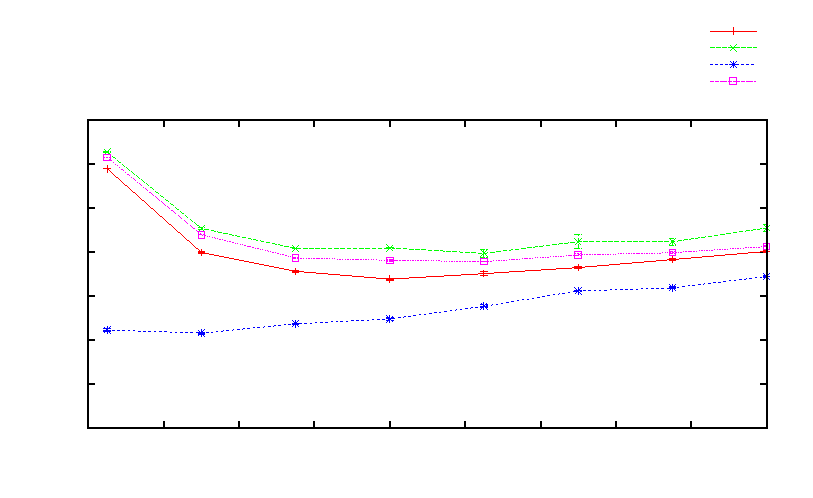
\includegraphics{PrecomputedRankBlockSize_Rank_TotalCycles}}%
    \gplfronttext
  \end{picture}%
\endgroup

\figureEnd

\figureBegin
\caption{Branch Mispredictions for Rank queries on wavelet trees with precomputed ranks of varying block sizes}
\label{fig:PrecomputedRankBlockSize_Rank_BranchMiss}
% GNUPLOT: LaTeX picture with Postscript
\begingroup
  \makeatletter
  \providecommand\color[2][]{%
    \GenericError{(gnuplot) \space\space\space\@spaces}{%
      Package color not loaded in conjunction with
      terminal option `colourtext'%
    }{See the gnuplot documentation for explanation.%
    }{Either use 'blacktext' in gnuplot or load the package
      color.sty in LaTeX.}%
    \renewcommand\color[2][]{}%
  }%
  \providecommand\includegraphics[2][]{%
    \GenericError{(gnuplot) \space\space\space\@spaces}{%
      Package graphicx or graphics not loaded%
    }{See the gnuplot documentation for explanation.%
    }{The gnuplot epslatex terminal needs graphicx.sty or graphics.sty.}%
    \renewcommand\includegraphics[2][]{}%
  }%
  \providecommand\rotatebox[2]{#2}%
  \@ifundefined{ifGPcolor}{%
    \newif\ifGPcolor
    \GPcolortrue
  }{}%
  \@ifundefined{ifGPblacktext}{%
    \newif\ifGPblacktext
    \GPblacktexttrue
  }{}%
  % define a \g@addto@macro without @ in the name:
  \let\gplgaddtomacro\g@addto@macro
  % define empty templates for all commands taking text:
  \gdef\gplbacktext{}%
  \gdef\gplfronttext{}%
  \makeatother
  \ifGPblacktext
    % no textcolor at all
    \def\colorrgb#1{}%
    \def\colorgray#1{}%
  \else
    % gray or color?
    \ifGPcolor
      \def\colorrgb#1{\color[rgb]{#1}}%
      \def\colorgray#1{\color[gray]{#1}}%
      \expandafter\def\csname LTw\endcsname{\color{white}}%
      \expandafter\def\csname LTb\endcsname{\color{black}}%
      \expandafter\def\csname LTa\endcsname{\color{black}}%
      \expandafter\def\csname LT0\endcsname{\color[rgb]{1,0,0}}%
      \expandafter\def\csname LT1\endcsname{\color[rgb]{0,1,0}}%
      \expandafter\def\csname LT2\endcsname{\color[rgb]{0,0,1}}%
      \expandafter\def\csname LT3\endcsname{\color[rgb]{1,0,1}}%
      \expandafter\def\csname LT4\endcsname{\color[rgb]{0,1,1}}%
      \expandafter\def\csname LT5\endcsname{\color[rgb]{1,1,0}}%
      \expandafter\def\csname LT6\endcsname{\color[rgb]{0,0,0}}%
      \expandafter\def\csname LT7\endcsname{\color[rgb]{1,0.3,0}}%
      \expandafter\def\csname LT8\endcsname{\color[rgb]{0.5,0.5,0.5}}%
    \else
      % gray
      \def\colorrgb#1{\color{black}}%
      \def\colorgray#1{\color[gray]{#1}}%
      \expandafter\def\csname LTw\endcsname{\color{white}}%
      \expandafter\def\csname LTb\endcsname{\color{black}}%
      \expandafter\def\csname LTa\endcsname{\color{black}}%
      \expandafter\def\csname LT0\endcsname{\color{black}}%
      \expandafter\def\csname LT1\endcsname{\color{black}}%
      \expandafter\def\csname LT2\endcsname{\color{black}}%
      \expandafter\def\csname LT3\endcsname{\color{black}}%
      \expandafter\def\csname LT4\endcsname{\color{black}}%
      \expandafter\def\csname LT5\endcsname{\color{black}}%
      \expandafter\def\csname LT6\endcsname{\color{black}}%
      \expandafter\def\csname LT7\endcsname{\color{black}}%
      \expandafter\def\csname LT8\endcsname{\color{black}}%
    \fi
  \fi
  \setlength{\unitlength}{0.0500bp}%
  \begin{picture}(7488.00,4464.00)%
    \gplgaddtomacro\gplbacktext{%
      \csname LTb\endcsname%
      \put(1210,704){\makebox(0,0)[r]{\strut{} 0}}%
      \put(1210,1078){\makebox(0,0)[r]{\strut{} 10000}}%
      \put(1210,1451){\makebox(0,0)[r]{\strut{} 20000}}%
      \put(1210,1825){\makebox(0,0)[r]{\strut{} 30000}}%
      \put(1210,2198){\makebox(0,0)[r]{\strut{} 40000}}%
      \put(1210,2572){\makebox(0,0)[r]{\strut{} 50000}}%
      \put(1210,2945){\makebox(0,0)[r]{\strut{} 60000}}%
      \put(1210,3319){\makebox(0,0)[r]{\strut{} 70000}}%
      \put(1342,484){\makebox(0,0){\strut{} 0.2}}%
      \put(1981,484){\makebox(0,0){\strut{} 0.4}}%
      \put(2620,484){\makebox(0,0){\strut{} 0.6}}%
      \put(3258,484){\makebox(0,0){\strut{} 0.8}}%
      \put(3897,484){\makebox(0,0){\strut{} 1}}%
      \put(4536,484){\makebox(0,0){\strut{} 1.2}}%
      \put(5175,484){\makebox(0,0){\strut{} 1.4}}%
      \put(5813,484){\makebox(0,0){\strut{} 1.6}}%
      \put(6452,484){\makebox(0,0){\strut{} 1.8}}%
      \put(7091,484){\makebox(0,0){\strut{} 2}}%
      \put(176,2011){\rotatebox{-270}{\makebox(0,0){\strut{}Branch Mispredictions}}}%
      \put(4216,154){\makebox(0,0){\strut{}Block Size (number of pages)}}%
    }%
    \gplgaddtomacro\gplfronttext{%
      \csname LTb\endcsname%
      \put(6468,4291){\makebox(0,0)[r]{\strut{}NaivePrecomputed, $mr\hat{\sigma}=$ 0.52 $avg\hat{\sigma}=$ 0.29}}%
      \csname LTb\endcsname%
      \put(6468,4071){\makebox(0,0)[r]{\strut{}PreallocatedPrecomputed, $mr\hat{\sigma}=$ 0.69 $avg\hat{\sigma}=$ 0.36}}%
      \csname LTb\endcsname%
      \put(6468,3851){\makebox(0,0)[r]{\strut{}UnalignedNaivePrecomputed, $mr\hat{\sigma}=$ 0.84 $avg\hat{\sigma}=$ 0.60}}%
    }%
    \gplbacktext
    \put(0,0){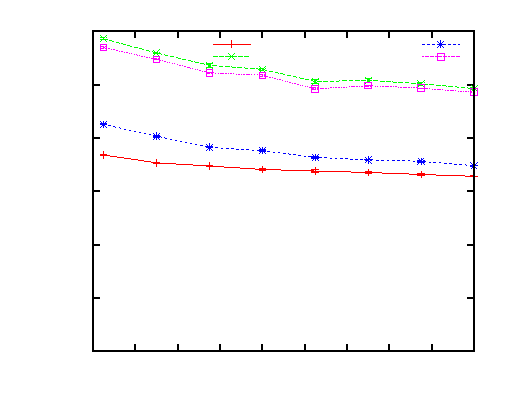
\includegraphics{PrecomputedRankBlockSize_Rank_BranchMiss}}%
    \gplfronttext
  \end{picture}%
\endgroup

\figureEnd


\figureBegin
\caption{Branch Misprediction Rate for Rank queries on wavelet trees with precomputed ranks of varying block sizes}
\label{fig:PrecomputedRankBlockSize_Rank_BranchMissRate}
% GNUPLOT: LaTeX picture with Postscript
\begingroup
  \makeatletter
  \providecommand\color[2][]{%
    \GenericError{(gnuplot) \space\space\space\@spaces}{%
      Package color not loaded in conjunction with
      terminal option `colourtext'%
    }{See the gnuplot documentation for explanation.%
    }{Either use 'blacktext' in gnuplot or load the package
      color.sty in LaTeX.}%
    \renewcommand\color[2][]{}%
  }%
  \providecommand\includegraphics[2][]{%
    \GenericError{(gnuplot) \space\space\space\@spaces}{%
      Package graphicx or graphics not loaded%
    }{See the gnuplot documentation for explanation.%
    }{The gnuplot epslatex terminal needs graphicx.sty or graphics.sty.}%
    \renewcommand\includegraphics[2][]{}%
  }%
  \providecommand\rotatebox[2]{#2}%
  \@ifundefined{ifGPcolor}{%
    \newif\ifGPcolor
    \GPcolortrue
  }{}%
  \@ifundefined{ifGPblacktext}{%
    \newif\ifGPblacktext
    \GPblacktexttrue
  }{}%
  % define a \g@addto@macro without @ in the name:
  \let\gplgaddtomacro\g@addto@macro
  % define empty templates for all commands taking text:
  \gdef\gplbacktext{}%
  \gdef\gplfronttext{}%
  \makeatother
  \ifGPblacktext
    % no textcolor at all
    \def\colorrgb#1{}%
    \def\colorgray#1{}%
  \else
    % gray or color?
    \ifGPcolor
      \def\colorrgb#1{\color[rgb]{#1}}%
      \def\colorgray#1{\color[gray]{#1}}%
      \expandafter\def\csname LTw\endcsname{\color{white}}%
      \expandafter\def\csname LTb\endcsname{\color{black}}%
      \expandafter\def\csname LTa\endcsname{\color{black}}%
      \expandafter\def\csname LT0\endcsname{\color[rgb]{1,0,0}}%
      \expandafter\def\csname LT1\endcsname{\color[rgb]{0,1,0}}%
      \expandafter\def\csname LT2\endcsname{\color[rgb]{0,0,1}}%
      \expandafter\def\csname LT3\endcsname{\color[rgb]{1,0,1}}%
      \expandafter\def\csname LT4\endcsname{\color[rgb]{0,1,1}}%
      \expandafter\def\csname LT5\endcsname{\color[rgb]{1,1,0}}%
      \expandafter\def\csname LT6\endcsname{\color[rgb]{0,0,0}}%
      \expandafter\def\csname LT7\endcsname{\color[rgb]{1,0.3,0}}%
      \expandafter\def\csname LT8\endcsname{\color[rgb]{0.5,0.5,0.5}}%
    \else
      % gray
      \def\colorrgb#1{\color{black}}%
      \def\colorgray#1{\color[gray]{#1}}%
      \expandafter\def\csname LTw\endcsname{\color{white}}%
      \expandafter\def\csname LTb\endcsname{\color{black}}%
      \expandafter\def\csname LTa\endcsname{\color{black}}%
      \expandafter\def\csname LT0\endcsname{\color{black}}%
      \expandafter\def\csname LT1\endcsname{\color{black}}%
      \expandafter\def\csname LT2\endcsname{\color{black}}%
      \expandafter\def\csname LT3\endcsname{\color{black}}%
      \expandafter\def\csname LT4\endcsname{\color{black}}%
      \expandafter\def\csname LT5\endcsname{\color{black}}%
      \expandafter\def\csname LT6\endcsname{\color{black}}%
      \expandafter\def\csname LT7\endcsname{\color{black}}%
      \expandafter\def\csname LT8\endcsname{\color{black}}%
    \fi
  \fi
  \setlength{\unitlength}{0.0500bp}%
  \begin{picture}(7488.00,4464.00)%
    \gplgaddtomacro\gplbacktext{%
      \csname LTb\endcsname%
      \put(1210,704){\makebox(0,0)[r]{\strut{} 0}}%
      \put(1210,966){\makebox(0,0)[r]{\strut{} 0.002}}%
      \put(1210,1227){\makebox(0,0)[r]{\strut{} 0.004}}%
      \put(1210,1489){\makebox(0,0)[r]{\strut{} 0.006}}%
      \put(1210,1750){\makebox(0,0)[r]{\strut{} 0.008}}%
      \put(1210,2012){\makebox(0,0)[r]{\strut{} 0.01}}%
      \put(1210,2273){\makebox(0,0)[r]{\strut{} 0.012}}%
      \put(1210,2535){\makebox(0,0)[r]{\strut{} 0.014}}%
      \put(1210,2796){\makebox(0,0)[r]{\strut{} 0.016}}%
      \put(1210,3058){\makebox(0,0)[r]{\strut{} 0.018}}%
      \put(1210,3319){\makebox(0,0)[r]{\strut{} 0.02}}%
      \put(1342,484){\makebox(0,0){\strut{} 0.2}}%
      \put(1981,484){\makebox(0,0){\strut{} 0.4}}%
      \put(2620,484){\makebox(0,0){\strut{} 0.6}}%
      \put(3258,484){\makebox(0,0){\strut{} 0.8}}%
      \put(3897,484){\makebox(0,0){\strut{} 1}}%
      \put(4536,484){\makebox(0,0){\strut{} 1.2}}%
      \put(5175,484){\makebox(0,0){\strut{} 1.4}}%
      \put(5813,484){\makebox(0,0){\strut{} 1.6}}%
      \put(6452,484){\makebox(0,0){\strut{} 1.8}}%
      \put(7091,484){\makebox(0,0){\strut{} 2}}%
      \put(176,2011){\rotatebox{-270}{\makebox(0,0){\strut{}Branch Misprediction Rate}}}%
      \put(4216,154){\makebox(0,0){\strut{}Block Size (number of pages)}}%
    }%
    \gplgaddtomacro\gplfronttext{%
      \csname LTb\endcsname%
      \put(6468,4291){\makebox(0,0)[r]{\strut{}NaivePrecomputed, $mr\hat{\sigma}=$ 1.44 $avg\hat{\sigma}=$ 0.63}}%
      \csname LTb\endcsname%
      \put(6468,4071){\makebox(0,0)[r]{\strut{}PreallocatedPrecomputed, $mr\hat{\sigma}=$ 4.24 $avg\hat{\sigma}=$ 1.43}}%
      \csname LTb\endcsname%
      \put(6468,3851){\makebox(0,0)[r]{\strut{}UnalignedNaivePrecomputed, $mr\hat{\sigma}=$ 0.84 $avg\hat{\sigma}=$ 0.60}}%
    }%
    \gplbacktext
    \put(0,0){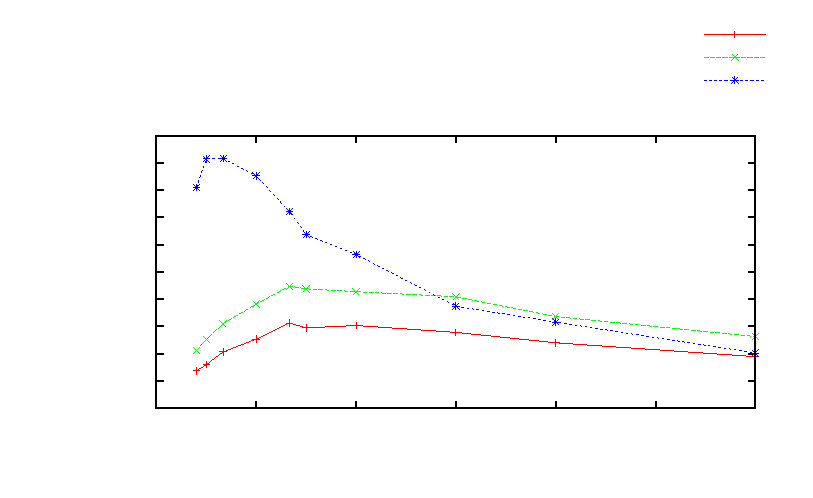
\includegraphics{PrecomputedRankBlockSize_Rank_BranchMissRate}}%
    \gplfronttext
  \end{picture}%
\endgroup

\figureEnd


\figureBegin
\caption{TLB Misses for Rank queries on wavelet trees with precomputed ranks of varying block sizes}
\label{fig:PrecomputedRankBlockSize_Rank_TLB}
% GNUPLOT: LaTeX picture with Postscript
\begingroup
  \makeatletter
  \providecommand\color[2][]{%
    \GenericError{(gnuplot) \space\space\space\@spaces}{%
      Package color not loaded in conjunction with
      terminal option `colourtext'%
    }{See the gnuplot documentation for explanation.%
    }{Either use 'blacktext' in gnuplot or load the package
      color.sty in LaTeX.}%
    \renewcommand\color[2][]{}%
  }%
  \providecommand\includegraphics[2][]{%
    \GenericError{(gnuplot) \space\space\space\@spaces}{%
      Package graphicx or graphics not loaded%
    }{See the gnuplot documentation for explanation.%
    }{The gnuplot epslatex terminal needs graphicx.sty or graphics.sty.}%
    \renewcommand\includegraphics[2][]{}%
  }%
  \providecommand\rotatebox[2]{#2}%
  \@ifundefined{ifGPcolor}{%
    \newif\ifGPcolor
    \GPcolortrue
  }{}%
  \@ifundefined{ifGPblacktext}{%
    \newif\ifGPblacktext
    \GPblacktexttrue
  }{}%
  % define a \g@addto@macro without @ in the name:
  \let\gplgaddtomacro\g@addto@macro
  % define empty templates for all commands taking text:
  \gdef\gplbacktext{}%
  \gdef\gplfronttext{}%
  \makeatother
  \ifGPblacktext
    % no textcolor at all
    \def\colorrgb#1{}%
    \def\colorgray#1{}%
  \else
    % gray or color?
    \ifGPcolor
      \def\colorrgb#1{\color[rgb]{#1}}%
      \def\colorgray#1{\color[gray]{#1}}%
      \expandafter\def\csname LTw\endcsname{\color{white}}%
      \expandafter\def\csname LTb\endcsname{\color{black}}%
      \expandafter\def\csname LTa\endcsname{\color{black}}%
      \expandafter\def\csname LT0\endcsname{\color[rgb]{1,0,0}}%
      \expandafter\def\csname LT1\endcsname{\color[rgb]{0,1,0}}%
      \expandafter\def\csname LT2\endcsname{\color[rgb]{0,0,1}}%
      \expandafter\def\csname LT3\endcsname{\color[rgb]{1,0,1}}%
      \expandafter\def\csname LT4\endcsname{\color[rgb]{0,1,1}}%
      \expandafter\def\csname LT5\endcsname{\color[rgb]{1,1,0}}%
      \expandafter\def\csname LT6\endcsname{\color[rgb]{0,0,0}}%
      \expandafter\def\csname LT7\endcsname{\color[rgb]{1,0.3,0}}%
      \expandafter\def\csname LT8\endcsname{\color[rgb]{0.5,0.5,0.5}}%
    \else
      % gray
      \def\colorrgb#1{\color{black}}%
      \def\colorgray#1{\color[gray]{#1}}%
      \expandafter\def\csname LTw\endcsname{\color{white}}%
      \expandafter\def\csname LTb\endcsname{\color{black}}%
      \expandafter\def\csname LTa\endcsname{\color{black}}%
      \expandafter\def\csname LT0\endcsname{\color{black}}%
      \expandafter\def\csname LT1\endcsname{\color{black}}%
      \expandafter\def\csname LT2\endcsname{\color{black}}%
      \expandafter\def\csname LT3\endcsname{\color{black}}%
      \expandafter\def\csname LT4\endcsname{\color{black}}%
      \expandafter\def\csname LT5\endcsname{\color{black}}%
      \expandafter\def\csname LT6\endcsname{\color{black}}%
      \expandafter\def\csname LT7\endcsname{\color{black}}%
      \expandafter\def\csname LT8\endcsname{\color{black}}%
    \fi
  \fi
  \setlength{\unitlength}{0.0500bp}%
  \begin{picture}(7488.00,4464.00)%
    \gplgaddtomacro\gplbacktext{%
      \csname LTb\endcsname%
      \put(1078,704){\makebox(0,0)[r]{\strut{} 0}}%
      \put(1078,1140){\makebox(0,0)[r]{\strut{} 1000}}%
      \put(1078,1576){\makebox(0,0)[r]{\strut{} 2000}}%
      \put(1078,2012){\makebox(0,0)[r]{\strut{} 3000}}%
      \put(1078,2447){\makebox(0,0)[r]{\strut{} 4000}}%
      \put(1078,2883){\makebox(0,0)[r]{\strut{} 5000}}%
      \put(1078,3319){\makebox(0,0)[r]{\strut{} 6000}}%
      \put(1210,484){\makebox(0,0){\strut{} 0.2}}%
      \put(1863,484){\makebox(0,0){\strut{} 0.4}}%
      \put(2517,484){\makebox(0,0){\strut{} 0.6}}%
      \put(3170,484){\makebox(0,0){\strut{} 0.8}}%
      \put(3824,484){\makebox(0,0){\strut{} 1}}%
      \put(4477,484){\makebox(0,0){\strut{} 1.2}}%
      \put(5131,484){\makebox(0,0){\strut{} 1.4}}%
      \put(5784,484){\makebox(0,0){\strut{} 1.6}}%
      \put(6438,484){\makebox(0,0){\strut{} 1.8}}%
      \put(7091,484){\makebox(0,0){\strut{} 2}}%
      \put(176,2011){\rotatebox{-270}{\makebox(0,0){\strut{}TLB Misses}}}%
      \put(4150,154){\makebox(0,0){\strut{}Block Size (number of pages)}}%
    }%
    \gplgaddtomacro\gplfronttext{%
      \csname LTb\endcsname%
      \put(6468,4291){\makebox(0,0)[r]{\strut{}NaivePrecomputed, $mr\hat{\sigma}=$ 6.69 $avg\hat{\sigma}=$ 4.08}}%
      \csname LTb\endcsname%
      \put(6468,4071){\makebox(0,0)[r]{\strut{}PreallocatedPrecomputed, $mr\hat{\sigma}=$ 25.75 $avg\hat{\sigma}=$ 16.34}}%
      \csname LTb\endcsname%
      \put(6468,3851){\makebox(0,0)[r]{\strut{}UnalignedNaivePrecomputed, $mr\hat{\sigma}=$ 5.78 $avg\hat{\sigma}=$ 3.89}}%
    }%
    \gplbacktext
    \put(0,0){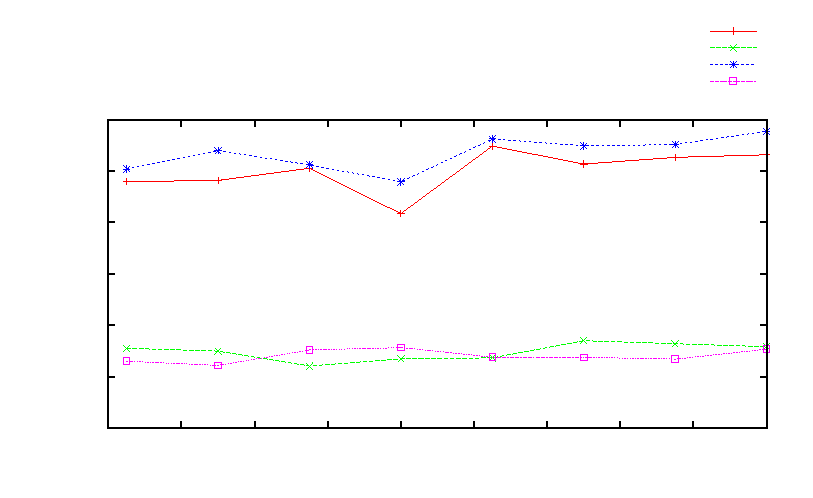
\includegraphics{PrecomputedRankBlockSize_Rank_TLB}}%
    \gplfronttext
  \end{picture}%
\endgroup

\figureEnd


\figureBegin
\caption{Level 1 Data Cache Misses for Rank queries on wavelet trees with precomputed ranks of varying block sizes}
\label{fig:PrecomputedRankBlockSize_Rank_L1CacheMiss}
% GNUPLOT: LaTeX picture with Postscript
\begingroup
  \makeatletter
  \providecommand\color[2][]{%
    \GenericError{(gnuplot) \space\space\space\@spaces}{%
      Package color not loaded in conjunction with
      terminal option `colourtext'%
    }{See the gnuplot documentation for explanation.%
    }{Either use 'blacktext' in gnuplot or load the package
      color.sty in LaTeX.}%
    \renewcommand\color[2][]{}%
  }%
  \providecommand\includegraphics[2][]{%
    \GenericError{(gnuplot) \space\space\space\@spaces}{%
      Package graphicx or graphics not loaded%
    }{See the gnuplot documentation for explanation.%
    }{The gnuplot epslatex terminal needs graphicx.sty or graphics.sty.}%
    \renewcommand\includegraphics[2][]{}%
  }%
  \providecommand\rotatebox[2]{#2}%
  \@ifundefined{ifGPcolor}{%
    \newif\ifGPcolor
    \GPcolortrue
  }{}%
  \@ifundefined{ifGPblacktext}{%
    \newif\ifGPblacktext
    \GPblacktexttrue
  }{}%
  % define a \g@addto@macro without @ in the name:
  \let\gplgaddtomacro\g@addto@macro
  % define empty templates for all commands taking text:
  \gdef\gplbacktext{}%
  \gdef\gplfronttext{}%
  \makeatother
  \ifGPblacktext
    % no textcolor at all
    \def\colorrgb#1{}%
    \def\colorgray#1{}%
  \else
    % gray or color?
    \ifGPcolor
      \def\colorrgb#1{\color[rgb]{#1}}%
      \def\colorgray#1{\color[gray]{#1}}%
      \expandafter\def\csname LTw\endcsname{\color{white}}%
      \expandafter\def\csname LTb\endcsname{\color{black}}%
      \expandafter\def\csname LTa\endcsname{\color{black}}%
      \expandafter\def\csname LT0\endcsname{\color[rgb]{1,0,0}}%
      \expandafter\def\csname LT1\endcsname{\color[rgb]{0,1,0}}%
      \expandafter\def\csname LT2\endcsname{\color[rgb]{0,0,1}}%
      \expandafter\def\csname LT3\endcsname{\color[rgb]{1,0,1}}%
      \expandafter\def\csname LT4\endcsname{\color[rgb]{0,1,1}}%
      \expandafter\def\csname LT5\endcsname{\color[rgb]{1,1,0}}%
      \expandafter\def\csname LT6\endcsname{\color[rgb]{0,0,0}}%
      \expandafter\def\csname LT7\endcsname{\color[rgb]{1,0.3,0}}%
      \expandafter\def\csname LT8\endcsname{\color[rgb]{0.5,0.5,0.5}}%
    \else
      % gray
      \def\colorrgb#1{\color{black}}%
      \def\colorgray#1{\color[gray]{#1}}%
      \expandafter\def\csname LTw\endcsname{\color{white}}%
      \expandafter\def\csname LTb\endcsname{\color{black}}%
      \expandafter\def\csname LTa\endcsname{\color{black}}%
      \expandafter\def\csname LT0\endcsname{\color{black}}%
      \expandafter\def\csname LT1\endcsname{\color{black}}%
      \expandafter\def\csname LT2\endcsname{\color{black}}%
      \expandafter\def\csname LT3\endcsname{\color{black}}%
      \expandafter\def\csname LT4\endcsname{\color{black}}%
      \expandafter\def\csname LT5\endcsname{\color{black}}%
      \expandafter\def\csname LT6\endcsname{\color{black}}%
      \expandafter\def\csname LT7\endcsname{\color{black}}%
      \expandafter\def\csname LT8\endcsname{\color{black}}%
    \fi
  \fi
  \setlength{\unitlength}{0.0500bp}%
  \begin{picture}(7488.00,4464.00)%
    \gplgaddtomacro\gplbacktext{%
      \csname LTb\endcsname%
      \put(1474,704){\makebox(0,0)[r]{\strut{} 0}}%
      \put(1474,1078){\makebox(0,0)[r]{\strut{} 200000}}%
      \put(1474,1451){\makebox(0,0)[r]{\strut{} 400000}}%
      \put(1474,1825){\makebox(0,0)[r]{\strut{} 600000}}%
      \put(1474,2198){\makebox(0,0)[r]{\strut{} 800000}}%
      \put(1474,2572){\makebox(0,0)[r]{\strut{} 1e+06}}%
      \put(1474,2945){\makebox(0,0)[r]{\strut{} 1.2e+06}}%
      \put(1474,3319){\makebox(0,0)[r]{\strut{} 1.4e+06}}%
      \put(1606,484){\makebox(0,0){\strut{} 0}}%
      \put(2520,484){\makebox(0,0){\strut{} 0.5}}%
      \put(3434,484){\makebox(0,0){\strut{} 1}}%
      \put(4349,484){\makebox(0,0){\strut{} 1.5}}%
      \put(5263,484){\makebox(0,0){\strut{} 2}}%
      \put(6177,484){\makebox(0,0){\strut{} 2.5}}%
      \put(7091,484){\makebox(0,0){\strut{} 3}}%
      \put(176,2011){\rotatebox{-270}{\makebox(0,0){\strut{}Cache Misses}}}%
      \put(4348,154){\makebox(0,0){\strut{}Block Size (number of pages)}}%
    }%
    \gplgaddtomacro\gplfronttext{%
      \csname LTb\endcsname%
      \put(6468,4291){\makebox(0,0)[r]{\strut{}NaivePrecomputed, $mr\hat{\sigma}=$ 1.67 $avg\hat{\sigma}=$ 0.55}}%
      \csname LTb\endcsname%
      \put(6468,4071){\makebox(0,0)[r]{\strut{}PreallocatedPrecomputed, $mr\hat{\sigma}=$ 5.27 $avg\hat{\sigma}=$ 1.63}}%
      \csname LTb\endcsname%
      \put(6468,3851){\makebox(0,0)[r]{\strut{}UnalignedNaivePrecomputed, $mr\hat{\sigma}=$ 0.17 $avg\hat{\sigma}=$ 0.09}}%
    }%
    \gplbacktext
    \put(0,0){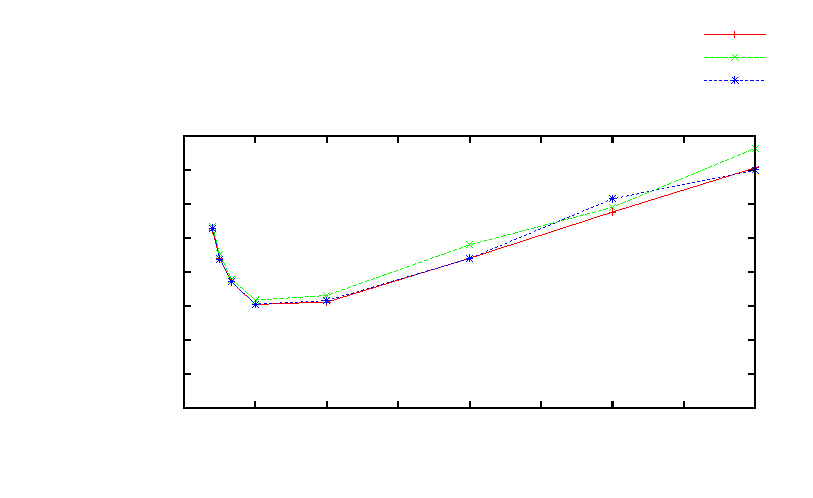
\includegraphics{PrecomputedRankBlockSize_Rank_L1CacheMiss}}%
    \gplfronttext
  \end{picture}%
\endgroup

\figureEnd


\figureBegin
\caption{Level 2 Data Cache Misses for Rank queries on wavelet trees with precomputed ranks of varying block sizes}
\label{fig:PrecomputedRankBlockSize_Rank_L2CacheMiss}
% GNUPLOT: LaTeX picture with Postscript
\begingroup
  \makeatletter
  \providecommand\color[2][]{%
    \GenericError{(gnuplot) \space\space\space\@spaces}{%
      Package color not loaded in conjunction with
      terminal option `colourtext'%
    }{See the gnuplot documentation for explanation.%
    }{Either use 'blacktext' in gnuplot or load the package
      color.sty in LaTeX.}%
    \renewcommand\color[2][]{}%
  }%
  \providecommand\includegraphics[2][]{%
    \GenericError{(gnuplot) \space\space\space\@spaces}{%
      Package graphicx or graphics not loaded%
    }{See the gnuplot documentation for explanation.%
    }{The gnuplot epslatex terminal needs graphicx.sty or graphics.sty.}%
    \renewcommand\includegraphics[2][]{}%
  }%
  \providecommand\rotatebox[2]{#2}%
  \@ifundefined{ifGPcolor}{%
    \newif\ifGPcolor
    \GPcolortrue
  }{}%
  \@ifundefined{ifGPblacktext}{%
    \newif\ifGPblacktext
    \GPblacktexttrue
  }{}%
  % define a \g@addto@macro without @ in the name:
  \let\gplgaddtomacro\g@addto@macro
  % define empty templates for all commands taking text:
  \gdef\gplbacktext{}%
  \gdef\gplfronttext{}%
  \makeatother
  \ifGPblacktext
    % no textcolor at all
    \def\colorrgb#1{}%
    \def\colorgray#1{}%
  \else
    % gray or color?
    \ifGPcolor
      \def\colorrgb#1{\color[rgb]{#1}}%
      \def\colorgray#1{\color[gray]{#1}}%
      \expandafter\def\csname LTw\endcsname{\color{white}}%
      \expandafter\def\csname LTb\endcsname{\color{black}}%
      \expandafter\def\csname LTa\endcsname{\color{black}}%
      \expandafter\def\csname LT0\endcsname{\color[rgb]{1,0,0}}%
      \expandafter\def\csname LT1\endcsname{\color[rgb]{0,1,0}}%
      \expandafter\def\csname LT2\endcsname{\color[rgb]{0,0,1}}%
      \expandafter\def\csname LT3\endcsname{\color[rgb]{1,0,1}}%
      \expandafter\def\csname LT4\endcsname{\color[rgb]{0,1,1}}%
      \expandafter\def\csname LT5\endcsname{\color[rgb]{1,1,0}}%
      \expandafter\def\csname LT6\endcsname{\color[rgb]{0,0,0}}%
      \expandafter\def\csname LT7\endcsname{\color[rgb]{1,0.3,0}}%
      \expandafter\def\csname LT8\endcsname{\color[rgb]{0.5,0.5,0.5}}%
    \else
      % gray
      \def\colorrgb#1{\color{black}}%
      \def\colorgray#1{\color[gray]{#1}}%
      \expandafter\def\csname LTw\endcsname{\color{white}}%
      \expandafter\def\csname LTb\endcsname{\color{black}}%
      \expandafter\def\csname LTa\endcsname{\color{black}}%
      \expandafter\def\csname LT0\endcsname{\color{black}}%
      \expandafter\def\csname LT1\endcsname{\color{black}}%
      \expandafter\def\csname LT2\endcsname{\color{black}}%
      \expandafter\def\csname LT3\endcsname{\color{black}}%
      \expandafter\def\csname LT4\endcsname{\color{black}}%
      \expandafter\def\csname LT5\endcsname{\color{black}}%
      \expandafter\def\csname LT6\endcsname{\color{black}}%
      \expandafter\def\csname LT7\endcsname{\color{black}}%
      \expandafter\def\csname LT8\endcsname{\color{black}}%
    \fi
  \fi
  \setlength{\unitlength}{0.0500bp}%
  \begin{picture}(4608.00,3600.00)%
    \gplgaddtomacro\gplbacktext{%
      \csname LTb\endcsname%
      \put(732,384){\makebox(0,0)[r]{\strut{} 0}}%
      \put(732,998){\makebox(0,0)[r]{\strut{} 50000}}%
      \put(732,1612){\makebox(0,0)[r]{\strut{} 100000}}%
      \put(732,2227){\makebox(0,0)[r]{\strut{} 150000}}%
      \put(732,2841){\makebox(0,0)[r]{\strut{} 200000}}%
      \put(732,3455){\makebox(0,0)[r]{\strut{} 250000}}%
      \put(804,264){\makebox(0,0){\strut{} 0.2}}%
      \put(1203,264){\makebox(0,0){\strut{} 0.4}}%
      \put(1601,264){\makebox(0,0){\strut{} 0.6}}%
      \put(2000,264){\makebox(0,0){\strut{} 0.8}}%
      \put(2398,264){\makebox(0,0){\strut{} 1}}%
      \put(2797,264){\makebox(0,0){\strut{} 1.2}}%
      \put(3195,264){\makebox(0,0){\strut{} 1.4}}%
      \put(3594,264){\makebox(0,0){\strut{} 1.6}}%
      \put(3992,264){\makebox(0,0){\strut{} 1.8}}%
      \put(4391,264){\makebox(0,0){\strut{} 2}}%
      \put(96,1919){\rotatebox{-270}{\makebox(0,0){\strut{}Cache Misses}}}%
      \put(2597,84){\makebox(0,0){\strut{}Block Size (number of pages)}}%
    }%
    \gplgaddtomacro\gplfronttext{%
      \csname LTb\endcsname%
      \put(1817,3332){\makebox(0,0)[r]{\strut{}Naive}}%
      \csname LTb\endcsname%
      \put(1817,3212){\makebox(0,0)[r]{\strut{}Preallocated}}%
      \csname LTb\endcsname%
      \put(3824,3332){\makebox(0,0)[r]{\strut{}UnalignedNaive}}%
      \csname LTb\endcsname%
      \put(3824,3212){\makebox(0,0)[r]{\strut{}UnalignedPreallocated}}%
    }%
    \gplbacktext
    \put(0,0){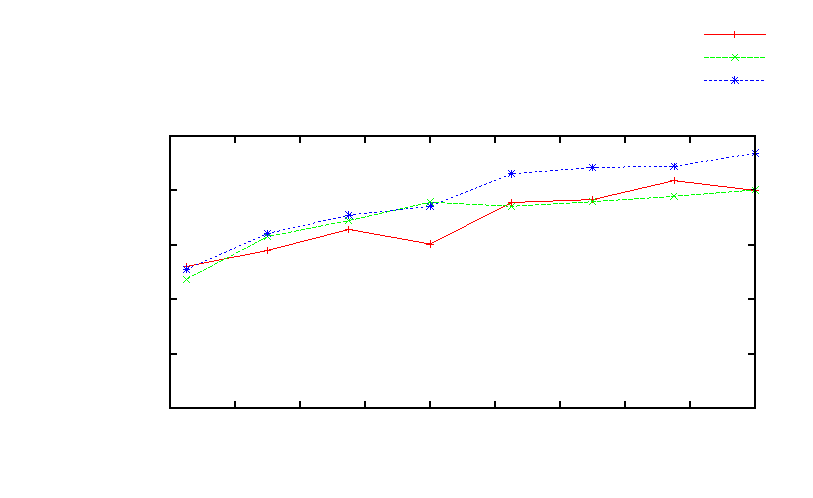
\includegraphics{PrecomputedRankBlockSize_Rank_L2CacheMiss}}%
    \gplfronttext
  \end{picture}%
\endgroup

\figureEnd


\figureBegin
\caption{Level 2 Data Cache Miss Rate for Rank queries on wavelet trees with precomputed ranks of varying block sizes}
\label{fig:PrecomputedRankBlockSize_Rank_L2CacheMissRate}
% GNUPLOT: LaTeX picture with Postscript
\begingroup
  \makeatletter
  \providecommand\color[2][]{%
    \GenericError{(gnuplot) \space\space\space\@spaces}{%
      Package color not loaded in conjunction with
      terminal option `colourtext'%
    }{See the gnuplot documentation for explanation.%
    }{Either use 'blacktext' in gnuplot or load the package
      color.sty in LaTeX.}%
    \renewcommand\color[2][]{}%
  }%
  \providecommand\includegraphics[2][]{%
    \GenericError{(gnuplot) \space\space\space\@spaces}{%
      Package graphicx or graphics not loaded%
    }{See the gnuplot documentation for explanation.%
    }{The gnuplot epslatex terminal needs graphicx.sty or graphics.sty.}%
    \renewcommand\includegraphics[2][]{}%
  }%
  \providecommand\rotatebox[2]{#2}%
  \@ifundefined{ifGPcolor}{%
    \newif\ifGPcolor
    \GPcolortrue
  }{}%
  \@ifundefined{ifGPblacktext}{%
    \newif\ifGPblacktext
    \GPblacktexttrue
  }{}%
  % define a \g@addto@macro without @ in the name:
  \let\gplgaddtomacro\g@addto@macro
  % define empty templates for all commands taking text:
  \gdef\gplbacktext{}%
  \gdef\gplfronttext{}%
  \makeatother
  \ifGPblacktext
    % no textcolor at all
    \def\colorrgb#1{}%
    \def\colorgray#1{}%
  \else
    % gray or color?
    \ifGPcolor
      \def\colorrgb#1{\color[rgb]{#1}}%
      \def\colorgray#1{\color[gray]{#1}}%
      \expandafter\def\csname LTw\endcsname{\color{white}}%
      \expandafter\def\csname LTb\endcsname{\color{black}}%
      \expandafter\def\csname LTa\endcsname{\color{black}}%
      \expandafter\def\csname LT0\endcsname{\color[rgb]{1,0,0}}%
      \expandafter\def\csname LT1\endcsname{\color[rgb]{0,1,0}}%
      \expandafter\def\csname LT2\endcsname{\color[rgb]{0,0,1}}%
      \expandafter\def\csname LT3\endcsname{\color[rgb]{1,0,1}}%
      \expandafter\def\csname LT4\endcsname{\color[rgb]{0,1,1}}%
      \expandafter\def\csname LT5\endcsname{\color[rgb]{1,1,0}}%
      \expandafter\def\csname LT6\endcsname{\color[rgb]{0,0,0}}%
      \expandafter\def\csname LT7\endcsname{\color[rgb]{1,0.3,0}}%
      \expandafter\def\csname LT8\endcsname{\color[rgb]{0.5,0.5,0.5}}%
    \else
      % gray
      \def\colorrgb#1{\color{black}}%
      \def\colorgray#1{\color[gray]{#1}}%
      \expandafter\def\csname LTw\endcsname{\color{white}}%
      \expandafter\def\csname LTb\endcsname{\color{black}}%
      \expandafter\def\csname LTa\endcsname{\color{black}}%
      \expandafter\def\csname LT0\endcsname{\color{black}}%
      \expandafter\def\csname LT1\endcsname{\color{black}}%
      \expandafter\def\csname LT2\endcsname{\color{black}}%
      \expandafter\def\csname LT3\endcsname{\color{black}}%
      \expandafter\def\csname LT4\endcsname{\color{black}}%
      \expandafter\def\csname LT5\endcsname{\color{black}}%
      \expandafter\def\csname LT6\endcsname{\color{black}}%
      \expandafter\def\csname LT7\endcsname{\color{black}}%
      \expandafter\def\csname LT8\endcsname{\color{black}}%
    \fi
  \fi
  \setlength{\unitlength}{0.0500bp}%
  \begin{picture}(7488.00,4464.00)%
    \gplgaddtomacro\gplbacktext{%
      \csname LTb\endcsname%
      \put(1078,704){\makebox(0,0)[r]{\strut{} 0}}%
      \put(1078,1031){\makebox(0,0)[r]{\strut{} 0.05}}%
      \put(1078,1358){\makebox(0,0)[r]{\strut{} 0.1}}%
      \put(1078,1685){\makebox(0,0)[r]{\strut{} 0.15}}%
      \put(1078,2012){\makebox(0,0)[r]{\strut{} 0.2}}%
      \put(1078,2338){\makebox(0,0)[r]{\strut{} 0.25}}%
      \put(1078,2665){\makebox(0,0)[r]{\strut{} 0.3}}%
      \put(1078,2992){\makebox(0,0)[r]{\strut{} 0.35}}%
      \put(1078,3319){\makebox(0,0)[r]{\strut{} 0.4}}%
      \put(1210,484){\makebox(0,0){\strut{} 0.2}}%
      \put(1863,484){\makebox(0,0){\strut{} 0.4}}%
      \put(2517,484){\makebox(0,0){\strut{} 0.6}}%
      \put(3170,484){\makebox(0,0){\strut{} 0.8}}%
      \put(3824,484){\makebox(0,0){\strut{} 1}}%
      \put(4477,484){\makebox(0,0){\strut{} 1.2}}%
      \put(5131,484){\makebox(0,0){\strut{} 1.4}}%
      \put(5784,484){\makebox(0,0){\strut{} 1.6}}%
      \put(6438,484){\makebox(0,0){\strut{} 1.8}}%
      \put(7091,484){\makebox(0,0){\strut{} 2}}%
      \put(176,2011){\rotatebox{-270}{\makebox(0,0){\strut{}Cache Miss Rate}}}%
      \put(4150,154){\makebox(0,0){\strut{}Block Size (number of pages)}}%
    }%
    \gplgaddtomacro\gplfronttext{%
      \csname LTb\endcsname%
      \put(6468,4291){\makebox(0,0)[r]{\strut{}NaivePrecomputed, $mr\hat{\sigma}=$ 0.38 $avg\hat{\sigma}=$ 0.38}}%
      \csname LTb\endcsname%
      \put(6468,4071){\makebox(0,0)[r]{\strut{}PreallocatedPrecomputed, $mr\hat{\sigma}=$ 0.26 $avg\hat{\sigma}=$ 0.26}}%
      \csname LTb\endcsname%
      \put(6468,3851){\makebox(0,0)[r]{\strut{}UnalignedNaivePrecomputed, $mr\hat{\sigma}=$ 0.72 $avg\hat{\sigma}=$ 0.62}}%
    }%
    \gplbacktext
    \put(0,0){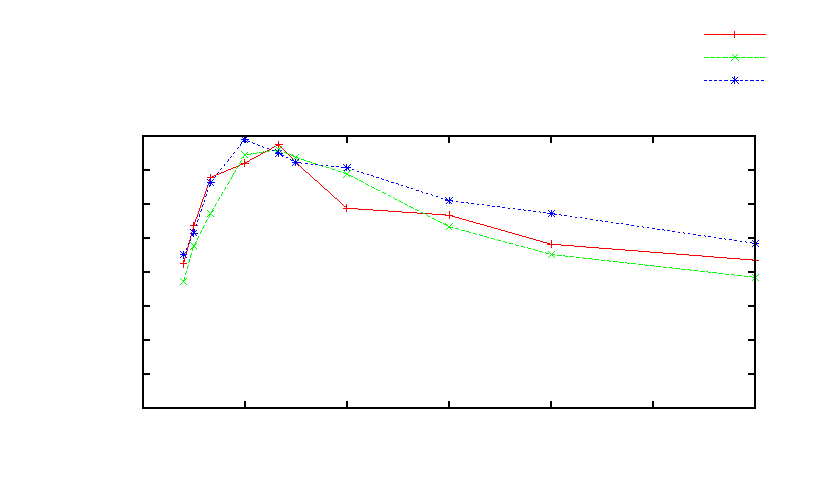
\includegraphics{PrecomputedRankBlockSize_Rank_L2CacheMissRate}}%
    \gplfronttext
  \end{picture}%
\endgroup

\figureEnd


\figureBegin
\caption{Level 3 Total Cache Misses for Rank queries on wavelet trees with precomputed ranks of varying block sizes}
\label{fig:PrecomputedRankBlockSize_Rank_L3CacheMiss}
% GNUPLOT: LaTeX picture with Postscript
\begingroup
  \makeatletter
  \providecommand\color[2][]{%
    \GenericError{(gnuplot) \space\space\space\@spaces}{%
      Package color not loaded in conjunction with
      terminal option `colourtext'%
    }{See the gnuplot documentation for explanation.%
    }{Either use 'blacktext' in gnuplot or load the package
      color.sty in LaTeX.}%
    \renewcommand\color[2][]{}%
  }%
  \providecommand\includegraphics[2][]{%
    \GenericError{(gnuplot) \space\space\space\@spaces}{%
      Package graphicx or graphics not loaded%
    }{See the gnuplot documentation for explanation.%
    }{The gnuplot epslatex terminal needs graphicx.sty or graphics.sty.}%
    \renewcommand\includegraphics[2][]{}%
  }%
  \providecommand\rotatebox[2]{#2}%
  \@ifundefined{ifGPcolor}{%
    \newif\ifGPcolor
    \GPcolortrue
  }{}%
  \@ifundefined{ifGPblacktext}{%
    \newif\ifGPblacktext
    \GPblacktexttrue
  }{}%
  % define a \g@addto@macro without @ in the name:
  \let\gplgaddtomacro\g@addto@macro
  % define empty templates for all commands taking text:
  \gdef\gplbacktext{}%
  \gdef\gplfronttext{}%
  \makeatother
  \ifGPblacktext
    % no textcolor at all
    \def\colorrgb#1{}%
    \def\colorgray#1{}%
  \else
    % gray or color?
    \ifGPcolor
      \def\colorrgb#1{\color[rgb]{#1}}%
      \def\colorgray#1{\color[gray]{#1}}%
      \expandafter\def\csname LTw\endcsname{\color{white}}%
      \expandafter\def\csname LTb\endcsname{\color{black}}%
      \expandafter\def\csname LTa\endcsname{\color{black}}%
      \expandafter\def\csname LT0\endcsname{\color[rgb]{1,0,0}}%
      \expandafter\def\csname LT1\endcsname{\color[rgb]{0,1,0}}%
      \expandafter\def\csname LT2\endcsname{\color[rgb]{0,0,1}}%
      \expandafter\def\csname LT3\endcsname{\color[rgb]{1,0,1}}%
      \expandafter\def\csname LT4\endcsname{\color[rgb]{0,1,1}}%
      \expandafter\def\csname LT5\endcsname{\color[rgb]{1,1,0}}%
      \expandafter\def\csname LT6\endcsname{\color[rgb]{0,0,0}}%
      \expandafter\def\csname LT7\endcsname{\color[rgb]{1,0.3,0}}%
      \expandafter\def\csname LT8\endcsname{\color[rgb]{0.5,0.5,0.5}}%
    \else
      % gray
      \def\colorrgb#1{\color{black}}%
      \def\colorgray#1{\color[gray]{#1}}%
      \expandafter\def\csname LTw\endcsname{\color{white}}%
      \expandafter\def\csname LTb\endcsname{\color{black}}%
      \expandafter\def\csname LTa\endcsname{\color{black}}%
      \expandafter\def\csname LT0\endcsname{\color{black}}%
      \expandafter\def\csname LT1\endcsname{\color{black}}%
      \expandafter\def\csname LT2\endcsname{\color{black}}%
      \expandafter\def\csname LT3\endcsname{\color{black}}%
      \expandafter\def\csname LT4\endcsname{\color{black}}%
      \expandafter\def\csname LT5\endcsname{\color{black}}%
      \expandafter\def\csname LT6\endcsname{\color{black}}%
      \expandafter\def\csname LT7\endcsname{\color{black}}%
      \expandafter\def\csname LT8\endcsname{\color{black}}%
    \fi
  \fi
  \setlength{\unitlength}{0.0500bp}%
  \begin{picture}(4608.00,3600.00)%
    \gplgaddtomacro\gplbacktext{%
      \csname LTb\endcsname%
      \put(732,384){\makebox(0,0)[r]{\strut{} 0}}%
      \put(732,768){\makebox(0,0)[r]{\strut{} 20000}}%
      \put(732,1152){\makebox(0,0)[r]{\strut{} 40000}}%
      \put(732,1536){\makebox(0,0)[r]{\strut{} 60000}}%
      \put(732,1920){\makebox(0,0)[r]{\strut{} 80000}}%
      \put(732,2303){\makebox(0,0)[r]{\strut{} 100000}}%
      \put(732,2687){\makebox(0,0)[r]{\strut{} 120000}}%
      \put(732,3071){\makebox(0,0)[r]{\strut{} 140000}}%
      \put(732,3455){\makebox(0,0)[r]{\strut{} 160000}}%
      \put(804,264){\makebox(0,0){\strut{} 0.2}}%
      \put(1203,264){\makebox(0,0){\strut{} 0.4}}%
      \put(1601,264){\makebox(0,0){\strut{} 0.6}}%
      \put(2000,264){\makebox(0,0){\strut{} 0.8}}%
      \put(2398,264){\makebox(0,0){\strut{} 1}}%
      \put(2797,264){\makebox(0,0){\strut{} 1.2}}%
      \put(3195,264){\makebox(0,0){\strut{} 1.4}}%
      \put(3594,264){\makebox(0,0){\strut{} 1.6}}%
      \put(3992,264){\makebox(0,0){\strut{} 1.8}}%
      \put(4391,264){\makebox(0,0){\strut{} 2}}%
      \put(96,1919){\rotatebox{-270}{\makebox(0,0){\strut{}Cache Misses}}}%
      \put(2597,84){\makebox(0,0){\strut{}Block Size (number of pages)}}%
    }%
    \gplgaddtomacro\gplfronttext{%
      \csname LTb\endcsname%
      \put(1817,3332){\makebox(0,0)[r]{\strut{}Naive}}%
      \csname LTb\endcsname%
      \put(1817,3212){\makebox(0,0)[r]{\strut{}Preallocated}}%
      \csname LTb\endcsname%
      \put(3824,3332){\makebox(0,0)[r]{\strut{}UnalignedNaive}}%
      \csname LTb\endcsname%
      \put(3824,3212){\makebox(0,0)[r]{\strut{}UnalignedPreallocated}}%
    }%
    \gplbacktext
    \put(0,0){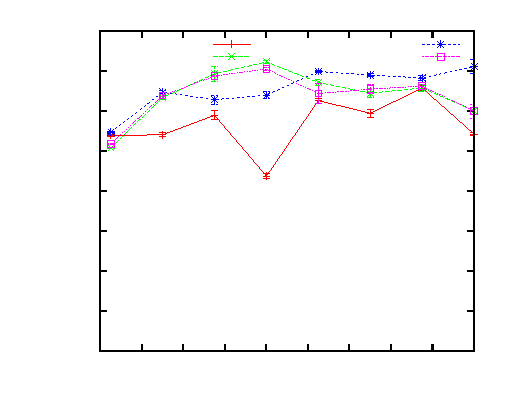
\includegraphics{PrecomputedRankBlockSize_Rank_L3CacheMiss}}%
    \gplfronttext
  \end{picture}%
\endgroup

\figureEnd




\clearpage



\paragraph{Select Queries}~\\


\figureBegin
\caption{Wall Time of Select queries on wavelet trees with precomputed ranks of varying block sizes}
\label{fig:PrecomputedRankBlockSize_Select_WallTime}
% GNUPLOT: LaTeX picture with Postscript
\begingroup
  \makeatletter
  \providecommand\color[2][]{%
    \GenericError{(gnuplot) \space\space\space\@spaces}{%
      Package color not loaded in conjunction with
      terminal option `colourtext'%
    }{See the gnuplot documentation for explanation.%
    }{Either use 'blacktext' in gnuplot or load the package
      color.sty in LaTeX.}%
    \renewcommand\color[2][]{}%
  }%
  \providecommand\includegraphics[2][]{%
    \GenericError{(gnuplot) \space\space\space\@spaces}{%
      Package graphicx or graphics not loaded%
    }{See the gnuplot documentation for explanation.%
    }{The gnuplot epslatex terminal needs graphicx.sty or graphics.sty.}%
    \renewcommand\includegraphics[2][]{}%
  }%
  \providecommand\rotatebox[2]{#2}%
  \@ifundefined{ifGPcolor}{%
    \newif\ifGPcolor
    \GPcolortrue
  }{}%
  \@ifundefined{ifGPblacktext}{%
    \newif\ifGPblacktext
    \GPblacktexttrue
  }{}%
  % define a \g@addto@macro without @ in the name:
  \let\gplgaddtomacro\g@addto@macro
  % define empty templates for all commands taking text:
  \gdef\gplbacktext{}%
  \gdef\gplfronttext{}%
  \makeatother
  \ifGPblacktext
    % no textcolor at all
    \def\colorrgb#1{}%
    \def\colorgray#1{}%
  \else
    % gray or color?
    \ifGPcolor
      \def\colorrgb#1{\color[rgb]{#1}}%
      \def\colorgray#1{\color[gray]{#1}}%
      \expandafter\def\csname LTw\endcsname{\color{white}}%
      \expandafter\def\csname LTb\endcsname{\color{black}}%
      \expandafter\def\csname LTa\endcsname{\color{black}}%
      \expandafter\def\csname LT0\endcsname{\color[rgb]{1,0,0}}%
      \expandafter\def\csname LT1\endcsname{\color[rgb]{0,1,0}}%
      \expandafter\def\csname LT2\endcsname{\color[rgb]{0,0,1}}%
      \expandafter\def\csname LT3\endcsname{\color[rgb]{1,0,1}}%
      \expandafter\def\csname LT4\endcsname{\color[rgb]{0,1,1}}%
      \expandafter\def\csname LT5\endcsname{\color[rgb]{1,1,0}}%
      \expandafter\def\csname LT6\endcsname{\color[rgb]{0,0,0}}%
      \expandafter\def\csname LT7\endcsname{\color[rgb]{1,0.3,0}}%
      \expandafter\def\csname LT8\endcsname{\color[rgb]{0.5,0.5,0.5}}%
    \else
      % gray
      \def\colorrgb#1{\color{black}}%
      \def\colorgray#1{\color[gray]{#1}}%
      \expandafter\def\csname LTw\endcsname{\color{white}}%
      \expandafter\def\csname LTb\endcsname{\color{black}}%
      \expandafter\def\csname LTa\endcsname{\color{black}}%
      \expandafter\def\csname LT0\endcsname{\color{black}}%
      \expandafter\def\csname LT1\endcsname{\color{black}}%
      \expandafter\def\csname LT2\endcsname{\color{black}}%
      \expandafter\def\csname LT3\endcsname{\color{black}}%
      \expandafter\def\csname LT4\endcsname{\color{black}}%
      \expandafter\def\csname LT5\endcsname{\color{black}}%
      \expandafter\def\csname LT6\endcsname{\color{black}}%
      \expandafter\def\csname LT7\endcsname{\color{black}}%
      \expandafter\def\csname LT8\endcsname{\color{black}}%
    \fi
  \fi
  \setlength{\unitlength}{0.0500bp}%
  \begin{picture}(7488.00,4464.00)%
    \gplgaddtomacro\gplbacktext{%
      \csname LTb\endcsname%
      \put(1210,704){\makebox(0,0)[r]{\strut{} 0}}%
      \put(1210,1227){\makebox(0,0)[r]{\strut{} 5000}}%
      \put(1210,1750){\makebox(0,0)[r]{\strut{} 10000}}%
      \put(1210,2273){\makebox(0,0)[r]{\strut{} 15000}}%
      \put(1210,2796){\makebox(0,0)[r]{\strut{} 20000}}%
      \put(1210,3319){\makebox(0,0)[r]{\strut{} 25000}}%
      \put(1342,484){\makebox(0,0){\strut{} 0}}%
      \put(2300,484){\makebox(0,0){\strut{} 0.5}}%
      \put(3258,484){\makebox(0,0){\strut{} 1}}%
      \put(4217,484){\makebox(0,0){\strut{} 1.5}}%
      \put(5175,484){\makebox(0,0){\strut{} 2}}%
      \put(6133,484){\makebox(0,0){\strut{} 2.5}}%
      \put(7091,484){\makebox(0,0){\strut{} 3}}%
      \put(176,2011){\rotatebox{-270}{\makebox(0,0){\strut{}Wall Time ($\mu s$)}}}%
      \put(4216,154){\makebox(0,0){\strut{}Block Size (number of pages)}}%
    }%
    \gplgaddtomacro\gplfronttext{%
      \csname LTb\endcsname%
      \put(6468,4291){\makebox(0,0)[r]{\strut{}NaivePrecomputed, $mr\hat{\sigma}=$ 1.76 $avg\hat{\sigma}=$ 0.81}}%
      \csname LTb\endcsname%
      \put(6468,4071){\makebox(0,0)[r]{\strut{}PreallocatedPrecomputed, $mr\hat{\sigma}=$ 1.13 $avg\hat{\sigma}=$ 0.41}}%
      \csname LTb\endcsname%
      \put(6468,3851){\makebox(0,0)[r]{\strut{}UnalignedNaivePrecomputed, $mr\hat{\sigma}=$ 2.07 $avg\hat{\sigma}=$ 0.66}}%
    }%
    \gplbacktext
    \put(0,0){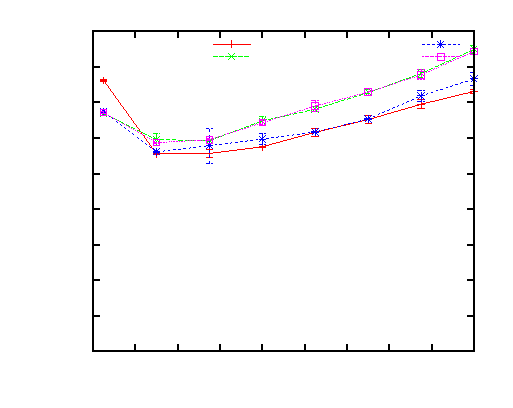
\includegraphics{PrecomputedRankBlockSize_Select_WallTime}}%
    \gplfronttext
  \end{picture}%
\endgroup

\figureEnd

\figureBegin
\caption{Branch Mispredictions for Select queries on wavelet trees with precomputed ranks of varying block sizes}
\label{fig:PrecomputedRankBlockSize_Select_BranchMiss}
% GNUPLOT: LaTeX picture with Postscript
\begingroup
  \makeatletter
  \providecommand\color[2][]{%
    \GenericError{(gnuplot) \space\space\space\@spaces}{%
      Package color not loaded in conjunction with
      terminal option `colourtext'%
    }{See the gnuplot documentation for explanation.%
    }{Either use 'blacktext' in gnuplot or load the package
      color.sty in LaTeX.}%
    \renewcommand\color[2][]{}%
  }%
  \providecommand\includegraphics[2][]{%
    \GenericError{(gnuplot) \space\space\space\@spaces}{%
      Package graphicx or graphics not loaded%
    }{See the gnuplot documentation for explanation.%
    }{The gnuplot epslatex terminal needs graphicx.sty or graphics.sty.}%
    \renewcommand\includegraphics[2][]{}%
  }%
  \providecommand\rotatebox[2]{#2}%
  \@ifundefined{ifGPcolor}{%
    \newif\ifGPcolor
    \GPcolortrue
  }{}%
  \@ifundefined{ifGPblacktext}{%
    \newif\ifGPblacktext
    \GPblacktexttrue
  }{}%
  % define a \g@addto@macro without @ in the name:
  \let\gplgaddtomacro\g@addto@macro
  % define empty templates for all commands taking text:
  \gdef\gplbacktext{}%
  \gdef\gplfronttext{}%
  \makeatother
  \ifGPblacktext
    % no textcolor at all
    \def\colorrgb#1{}%
    \def\colorgray#1{}%
  \else
    % gray or color?
    \ifGPcolor
      \def\colorrgb#1{\color[rgb]{#1}}%
      \def\colorgray#1{\color[gray]{#1}}%
      \expandafter\def\csname LTw\endcsname{\color{white}}%
      \expandafter\def\csname LTb\endcsname{\color{black}}%
      \expandafter\def\csname LTa\endcsname{\color{black}}%
      \expandafter\def\csname LT0\endcsname{\color[rgb]{1,0,0}}%
      \expandafter\def\csname LT1\endcsname{\color[rgb]{0,1,0}}%
      \expandafter\def\csname LT2\endcsname{\color[rgb]{0,0,1}}%
      \expandafter\def\csname LT3\endcsname{\color[rgb]{1,0,1}}%
      \expandafter\def\csname LT4\endcsname{\color[rgb]{0,1,1}}%
      \expandafter\def\csname LT5\endcsname{\color[rgb]{1,1,0}}%
      \expandafter\def\csname LT6\endcsname{\color[rgb]{0,0,0}}%
      \expandafter\def\csname LT7\endcsname{\color[rgb]{1,0.3,0}}%
      \expandafter\def\csname LT8\endcsname{\color[rgb]{0.5,0.5,0.5}}%
    \else
      % gray
      \def\colorrgb#1{\color{black}}%
      \def\colorgray#1{\color[gray]{#1}}%
      \expandafter\def\csname LTw\endcsname{\color{white}}%
      \expandafter\def\csname LTb\endcsname{\color{black}}%
      \expandafter\def\csname LTa\endcsname{\color{black}}%
      \expandafter\def\csname LT0\endcsname{\color{black}}%
      \expandafter\def\csname LT1\endcsname{\color{black}}%
      \expandafter\def\csname LT2\endcsname{\color{black}}%
      \expandafter\def\csname LT3\endcsname{\color{black}}%
      \expandafter\def\csname LT4\endcsname{\color{black}}%
      \expandafter\def\csname LT5\endcsname{\color{black}}%
      \expandafter\def\csname LT6\endcsname{\color{black}}%
      \expandafter\def\csname LT7\endcsname{\color{black}}%
      \expandafter\def\csname LT8\endcsname{\color{black}}%
    \fi
  \fi
  \setlength{\unitlength}{0.0500bp}%
  \begin{picture}(4608.00,3600.00)%
    \gplgaddtomacro\gplbacktext{%
      \csname LTb\endcsname%
      \put(732,384){\makebox(0,0)[r]{\strut{} 310000}}%
      \put(732,896){\makebox(0,0)[r]{\strut{} 315000}}%
      \put(732,1408){\makebox(0,0)[r]{\strut{} 320000}}%
      \put(732,1920){\makebox(0,0)[r]{\strut{} 325000}}%
      \put(732,2431){\makebox(0,0)[r]{\strut{} 330000}}%
      \put(732,2943){\makebox(0,0)[r]{\strut{} 335000}}%
      \put(732,3455){\makebox(0,0)[r]{\strut{} 340000}}%
      \put(804,264){\makebox(0,0){\strut{} 0.2}}%
      \put(1203,264){\makebox(0,0){\strut{} 0.4}}%
      \put(1601,264){\makebox(0,0){\strut{} 0.6}}%
      \put(2000,264){\makebox(0,0){\strut{} 0.8}}%
      \put(2398,264){\makebox(0,0){\strut{} 1}}%
      \put(2797,264){\makebox(0,0){\strut{} 1.2}}%
      \put(3195,264){\makebox(0,0){\strut{} 1.4}}%
      \put(3594,264){\makebox(0,0){\strut{} 1.6}}%
      \put(3992,264){\makebox(0,0){\strut{} 1.8}}%
      \put(4391,264){\makebox(0,0){\strut{} 2}}%
      \put(96,1919){\rotatebox{-270}{\makebox(0,0){\strut{}Branch Mispredictions}}}%
      \put(2597,84){\makebox(0,0){\strut{}Block Size (number of pages)}}%
    }%
    \gplgaddtomacro\gplfronttext{%
      \csname LTb\endcsname%
      \put(1817,3332){\makebox(0,0)[r]{\strut{}Naive}}%
      \csname LTb\endcsname%
      \put(1817,3212){\makebox(0,0)[r]{\strut{}Preallocated}}%
      \csname LTb\endcsname%
      \put(3824,3332){\makebox(0,0)[r]{\strut{}UnalignedNaive}}%
      \csname LTb\endcsname%
      \put(3824,3212){\makebox(0,0)[r]{\strut{}UnalignedPreallocated}}%
    }%
    \gplbacktext
    \put(0,0){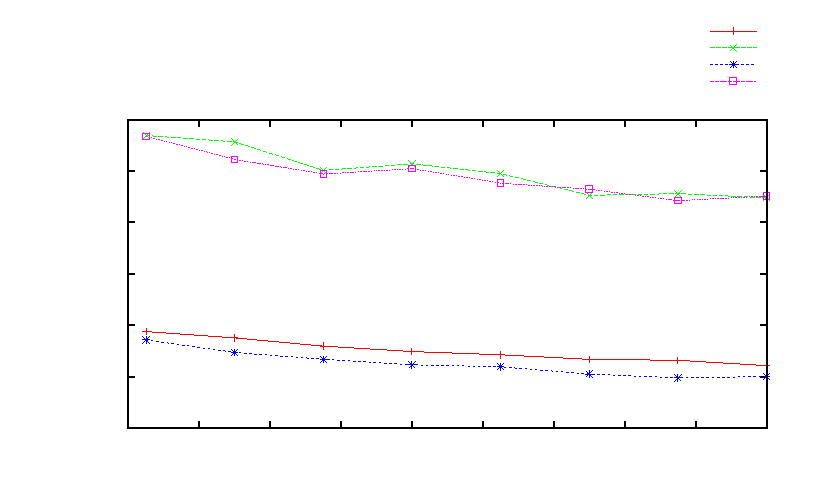
\includegraphics{PrecomputedRankBlockSize_Select_BranchMiss}}%
    \gplfronttext
  \end{picture}%
\endgroup

\figureEnd


\figureBegin
\caption{Branch Misprediction Rate for Select queries on wavelet trees with precomputed ranks of varying block sizes}
\label{fig:PrecomputedRankBlockSize_Select_BranchMissRate}
% GNUPLOT: LaTeX picture with Postscript
\begingroup
  \makeatletter
  \providecommand\color[2][]{%
    \GenericError{(gnuplot) \space\space\space\@spaces}{%
      Package color not loaded in conjunction with
      terminal option `colourtext'%
    }{See the gnuplot documentation for explanation.%
    }{Either use 'blacktext' in gnuplot or load the package
      color.sty in LaTeX.}%
    \renewcommand\color[2][]{}%
  }%
  \providecommand\includegraphics[2][]{%
    \GenericError{(gnuplot) \space\space\space\@spaces}{%
      Package graphicx or graphics not loaded%
    }{See the gnuplot documentation for explanation.%
    }{The gnuplot epslatex terminal needs graphicx.sty or graphics.sty.}%
    \renewcommand\includegraphics[2][]{}%
  }%
  \providecommand\rotatebox[2]{#2}%
  \@ifundefined{ifGPcolor}{%
    \newif\ifGPcolor
    \GPcolortrue
  }{}%
  \@ifundefined{ifGPblacktext}{%
    \newif\ifGPblacktext
    \GPblacktexttrue
  }{}%
  % define a \g@addto@macro without @ in the name:
  \let\gplgaddtomacro\g@addto@macro
  % define empty templates for all commands taking text:
  \gdef\gplbacktext{}%
  \gdef\gplfronttext{}%
  \makeatother
  \ifGPblacktext
    % no textcolor at all
    \def\colorrgb#1{}%
    \def\colorgray#1{}%
  \else
    % gray or color?
    \ifGPcolor
      \def\colorrgb#1{\color[rgb]{#1}}%
      \def\colorgray#1{\color[gray]{#1}}%
      \expandafter\def\csname LTw\endcsname{\color{white}}%
      \expandafter\def\csname LTb\endcsname{\color{black}}%
      \expandafter\def\csname LTa\endcsname{\color{black}}%
      \expandafter\def\csname LT0\endcsname{\color[rgb]{1,0,0}}%
      \expandafter\def\csname LT1\endcsname{\color[rgb]{0,1,0}}%
      \expandafter\def\csname LT2\endcsname{\color[rgb]{0,0,1}}%
      \expandafter\def\csname LT3\endcsname{\color[rgb]{1,0,1}}%
      \expandafter\def\csname LT4\endcsname{\color[rgb]{0,1,1}}%
      \expandafter\def\csname LT5\endcsname{\color[rgb]{1,1,0}}%
      \expandafter\def\csname LT6\endcsname{\color[rgb]{0,0,0}}%
      \expandafter\def\csname LT7\endcsname{\color[rgb]{1,0.3,0}}%
      \expandafter\def\csname LT8\endcsname{\color[rgb]{0.5,0.5,0.5}}%
    \else
      % gray
      \def\colorrgb#1{\color{black}}%
      \def\colorgray#1{\color[gray]{#1}}%
      \expandafter\def\csname LTw\endcsname{\color{white}}%
      \expandafter\def\csname LTb\endcsname{\color{black}}%
      \expandafter\def\csname LTa\endcsname{\color{black}}%
      \expandafter\def\csname LT0\endcsname{\color{black}}%
      \expandafter\def\csname LT1\endcsname{\color{black}}%
      \expandafter\def\csname LT2\endcsname{\color{black}}%
      \expandafter\def\csname LT3\endcsname{\color{black}}%
      \expandafter\def\csname LT4\endcsname{\color{black}}%
      \expandafter\def\csname LT5\endcsname{\color{black}}%
      \expandafter\def\csname LT6\endcsname{\color{black}}%
      \expandafter\def\csname LT7\endcsname{\color{black}}%
      \expandafter\def\csname LT8\endcsname{\color{black}}%
    \fi
  \fi
  \setlength{\unitlength}{0.0500bp}%
  \begin{picture}(7488.00,4464.00)%
    \gplgaddtomacro\gplbacktext{%
      \csname LTb\endcsname%
      \put(1210,704){\makebox(0,0)[r]{\strut{} 0}}%
      \put(1210,1140){\makebox(0,0)[r]{\strut{} 0.005}}%
      \put(1210,1576){\makebox(0,0)[r]{\strut{} 0.01}}%
      \put(1210,2012){\makebox(0,0)[r]{\strut{} 0.015}}%
      \put(1210,2447){\makebox(0,0)[r]{\strut{} 0.02}}%
      \put(1210,2883){\makebox(0,0)[r]{\strut{} 0.025}}%
      \put(1210,3319){\makebox(0,0)[r]{\strut{} 0.03}}%
      \put(1342,484){\makebox(0,0){\strut{} 0}}%
      \put(2061,484){\makebox(0,0){\strut{} 0.5}}%
      \put(2779,484){\makebox(0,0){\strut{} 1}}%
      \put(3498,484){\makebox(0,0){\strut{} 1.5}}%
      \put(4217,484){\makebox(0,0){\strut{} 2}}%
      \put(4935,484){\makebox(0,0){\strut{} 2.5}}%
      \put(5654,484){\makebox(0,0){\strut{} 3}}%
      \put(6372,484){\makebox(0,0){\strut{} 3.5}}%
      \put(7091,484){\makebox(0,0){\strut{} 4}}%
      \put(176,2011){\rotatebox{-270}{\makebox(0,0){\strut{}Cache Misses}}}%
      \put(4216,154){\makebox(0,0){\strut{}Block Size (number of pages)}}%
    }%
    \gplgaddtomacro\gplfronttext{%
      \csname LTb\endcsname%
      \put(6468,4291){\makebox(0,0)[r]{\strut{}NaivePrecomputed, $mr\hat{\sigma}=$ 0.62 $avg\hat{\sigma}=$ 0.32}}%
      \csname LTb\endcsname%
      \put(6468,4071){\makebox(0,0)[r]{\strut{}PreallocatedPrecomputed, $mr\hat{\sigma}=$ 2.20 $avg\hat{\sigma}=$ 0.53}}%
      \csname LTb\endcsname%
      \put(6468,3851){\makebox(0,0)[r]{\strut{}UnalignedNaivePrecomputed, $mr\hat{\sigma}=$ 0.12 $avg\hat{\sigma}=$ 0.08}}%
    }%
    \gplbacktext
    \put(0,0){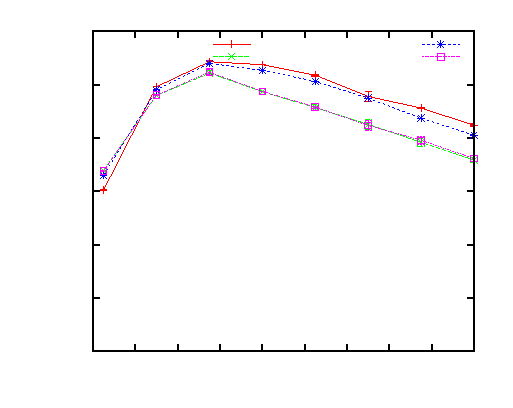
\includegraphics{PrecomputedRankBlockSize_Select_BranchMissRate}}%
    \gplfronttext
  \end{picture}%
\endgroup

\figureEnd


\figureBegin
\caption{TLB Misses for Select queries on wavelet trees with precomputed ranks of varying block sizes}
\label{fig:PrecomputedRankBlockSize_Select_TLB}
% GNUPLOT: LaTeX picture with Postscript
\begingroup
  \makeatletter
  \providecommand\color[2][]{%
    \GenericError{(gnuplot) \space\space\space\@spaces}{%
      Package color not loaded in conjunction with
      terminal option `colourtext'%
    }{See the gnuplot documentation for explanation.%
    }{Either use 'blacktext' in gnuplot or load the package
      color.sty in LaTeX.}%
    \renewcommand\color[2][]{}%
  }%
  \providecommand\includegraphics[2][]{%
    \GenericError{(gnuplot) \space\space\space\@spaces}{%
      Package graphicx or graphics not loaded%
    }{See the gnuplot documentation for explanation.%
    }{The gnuplot epslatex terminal needs graphicx.sty or graphics.sty.}%
    \renewcommand\includegraphics[2][]{}%
  }%
  \providecommand\rotatebox[2]{#2}%
  \@ifundefined{ifGPcolor}{%
    \newif\ifGPcolor
    \GPcolortrue
  }{}%
  \@ifundefined{ifGPblacktext}{%
    \newif\ifGPblacktext
    \GPblacktexttrue
  }{}%
  % define a \g@addto@macro without @ in the name:
  \let\gplgaddtomacro\g@addto@macro
  % define empty templates for all commands taking text:
  \gdef\gplbacktext{}%
  \gdef\gplfronttext{}%
  \makeatother
  \ifGPblacktext
    % no textcolor at all
    \def\colorrgb#1{}%
    \def\colorgray#1{}%
  \else
    % gray or color?
    \ifGPcolor
      \def\colorrgb#1{\color[rgb]{#1}}%
      \def\colorgray#1{\color[gray]{#1}}%
      \expandafter\def\csname LTw\endcsname{\color{white}}%
      \expandafter\def\csname LTb\endcsname{\color{black}}%
      \expandafter\def\csname LTa\endcsname{\color{black}}%
      \expandafter\def\csname LT0\endcsname{\color[rgb]{1,0,0}}%
      \expandafter\def\csname LT1\endcsname{\color[rgb]{0,1,0}}%
      \expandafter\def\csname LT2\endcsname{\color[rgb]{0,0,1}}%
      \expandafter\def\csname LT3\endcsname{\color[rgb]{1,0,1}}%
      \expandafter\def\csname LT4\endcsname{\color[rgb]{0,1,1}}%
      \expandafter\def\csname LT5\endcsname{\color[rgb]{1,1,0}}%
      \expandafter\def\csname LT6\endcsname{\color[rgb]{0,0,0}}%
      \expandafter\def\csname LT7\endcsname{\color[rgb]{1,0.3,0}}%
      \expandafter\def\csname LT8\endcsname{\color[rgb]{0.5,0.5,0.5}}%
    \else
      % gray
      \def\colorrgb#1{\color{black}}%
      \def\colorgray#1{\color[gray]{#1}}%
      \expandafter\def\csname LTw\endcsname{\color{white}}%
      \expandafter\def\csname LTb\endcsname{\color{black}}%
      \expandafter\def\csname LTa\endcsname{\color{black}}%
      \expandafter\def\csname LT0\endcsname{\color{black}}%
      \expandafter\def\csname LT1\endcsname{\color{black}}%
      \expandafter\def\csname LT2\endcsname{\color{black}}%
      \expandafter\def\csname LT3\endcsname{\color{black}}%
      \expandafter\def\csname LT4\endcsname{\color{black}}%
      \expandafter\def\csname LT5\endcsname{\color{black}}%
      \expandafter\def\csname LT6\endcsname{\color{black}}%
      \expandafter\def\csname LT7\endcsname{\color{black}}%
      \expandafter\def\csname LT8\endcsname{\color{black}}%
    \fi
  \fi
  \setlength{\unitlength}{0.0500bp}%
  \begin{picture}(7488.00,4464.00)%
    \gplgaddtomacro\gplbacktext{%
      \csname LTb\endcsname%
      \put(1078,704){\makebox(0,0)[r]{\strut{} 0}}%
      \put(1078,1031){\makebox(0,0)[r]{\strut{} 1000}}%
      \put(1078,1358){\makebox(0,0)[r]{\strut{} 2000}}%
      \put(1078,1685){\makebox(0,0)[r]{\strut{} 3000}}%
      \put(1078,2012){\makebox(0,0)[r]{\strut{} 4000}}%
      \put(1078,2338){\makebox(0,0)[r]{\strut{} 5000}}%
      \put(1078,2665){\makebox(0,0)[r]{\strut{} 6000}}%
      \put(1078,2992){\makebox(0,0)[r]{\strut{} 7000}}%
      \put(1078,3319){\makebox(0,0)[r]{\strut{} 8000}}%
      \put(1210,484){\makebox(0,0){\strut{} 0.2}}%
      \put(1863,484){\makebox(0,0){\strut{} 0.4}}%
      \put(2517,484){\makebox(0,0){\strut{} 0.6}}%
      \put(3170,484){\makebox(0,0){\strut{} 0.8}}%
      \put(3824,484){\makebox(0,0){\strut{} 1}}%
      \put(4477,484){\makebox(0,0){\strut{} 1.2}}%
      \put(5131,484){\makebox(0,0){\strut{} 1.4}}%
      \put(5784,484){\makebox(0,0){\strut{} 1.6}}%
      \put(6438,484){\makebox(0,0){\strut{} 1.8}}%
      \put(7091,484){\makebox(0,0){\strut{} 2}}%
      \put(176,2011){\rotatebox{-270}{\makebox(0,0){\strut{}TLB Misses}}}%
      \put(4150,154){\makebox(0,0){\strut{}Block Size (number of pages)}}%
    }%
    \gplgaddtomacro\gplfronttext{%
      \csname LTb\endcsname%
      \put(6468,4291){\makebox(0,0)[r]{\strut{}NaivePrecomputed, $mr\hat{\sigma}=$ 7.81 $avg\hat{\sigma}=$ 4.79}}%
      \csname LTb\endcsname%
      \put(6468,4071){\makebox(0,0)[r]{\strut{}PreallocatedPrecomputed, $mr\hat{\sigma}=$ 33.42 $avg\hat{\sigma}=$ 19.51}}%
      \csname LTb\endcsname%
      \put(6468,3851){\makebox(0,0)[r]{\strut{}UnalignedNaivePrecomputed, $mr\hat{\sigma}=$ 6.60 $avg\hat{\sigma}=$ 3.99}}%
    }%
    \gplbacktext
    \put(0,0){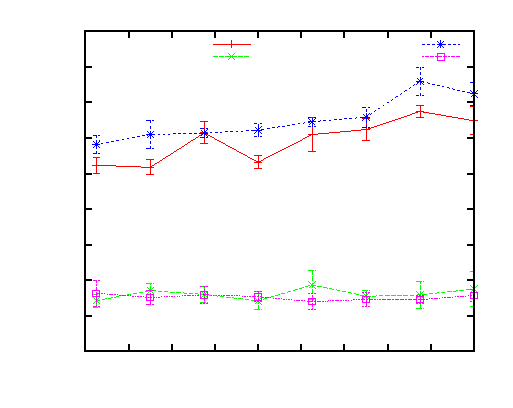
\includegraphics{PrecomputedRankBlockSize_Select_TLB}}%
    \gplfronttext
  \end{picture}%
\endgroup

\figureEnd


\figureBegin
\caption{Level 1 Data Cache Misses for Select queries on wavelet trees with precomputed ranks of varying block sizes}
\label{fig:PrecomputedRankBlockSize_Select_L1CacheMiss}
% GNUPLOT: LaTeX picture with Postscript
\begingroup
  \makeatletter
  \providecommand\color[2][]{%
    \GenericError{(gnuplot) \space\space\space\@spaces}{%
      Package color not loaded in conjunction with
      terminal option `colourtext'%
    }{See the gnuplot documentation for explanation.%
    }{Either use 'blacktext' in gnuplot or load the package
      color.sty in LaTeX.}%
    \renewcommand\color[2][]{}%
  }%
  \providecommand\includegraphics[2][]{%
    \GenericError{(gnuplot) \space\space\space\@spaces}{%
      Package graphicx or graphics not loaded%
    }{See the gnuplot documentation for explanation.%
    }{The gnuplot epslatex terminal needs graphicx.sty or graphics.sty.}%
    \renewcommand\includegraphics[2][]{}%
  }%
  \providecommand\rotatebox[2]{#2}%
  \@ifundefined{ifGPcolor}{%
    \newif\ifGPcolor
    \GPcolortrue
  }{}%
  \@ifundefined{ifGPblacktext}{%
    \newif\ifGPblacktext
    \GPblacktexttrue
  }{}%
  % define a \g@addto@macro without @ in the name:
  \let\gplgaddtomacro\g@addto@macro
  % define empty templates for all commands taking text:
  \gdef\gplbacktext{}%
  \gdef\gplfronttext{}%
  \makeatother
  \ifGPblacktext
    % no textcolor at all
    \def\colorrgb#1{}%
    \def\colorgray#1{}%
  \else
    % gray or color?
    \ifGPcolor
      \def\colorrgb#1{\color[rgb]{#1}}%
      \def\colorgray#1{\color[gray]{#1}}%
      \expandafter\def\csname LTw\endcsname{\color{white}}%
      \expandafter\def\csname LTb\endcsname{\color{black}}%
      \expandafter\def\csname LTa\endcsname{\color{black}}%
      \expandafter\def\csname LT0\endcsname{\color[rgb]{1,0,0}}%
      \expandafter\def\csname LT1\endcsname{\color[rgb]{0,1,0}}%
      \expandafter\def\csname LT2\endcsname{\color[rgb]{0,0,1}}%
      \expandafter\def\csname LT3\endcsname{\color[rgb]{1,0,1}}%
      \expandafter\def\csname LT4\endcsname{\color[rgb]{0,1,1}}%
      \expandafter\def\csname LT5\endcsname{\color[rgb]{1,1,0}}%
      \expandafter\def\csname LT6\endcsname{\color[rgb]{0,0,0}}%
      \expandafter\def\csname LT7\endcsname{\color[rgb]{1,0.3,0}}%
      \expandafter\def\csname LT8\endcsname{\color[rgb]{0.5,0.5,0.5}}%
    \else
      % gray
      \def\colorrgb#1{\color{black}}%
      \def\colorgray#1{\color[gray]{#1}}%
      \expandafter\def\csname LTw\endcsname{\color{white}}%
      \expandafter\def\csname LTb\endcsname{\color{black}}%
      \expandafter\def\csname LTa\endcsname{\color{black}}%
      \expandafter\def\csname LT0\endcsname{\color{black}}%
      \expandafter\def\csname LT1\endcsname{\color{black}}%
      \expandafter\def\csname LT2\endcsname{\color{black}}%
      \expandafter\def\csname LT3\endcsname{\color{black}}%
      \expandafter\def\csname LT4\endcsname{\color{black}}%
      \expandafter\def\csname LT5\endcsname{\color{black}}%
      \expandafter\def\csname LT6\endcsname{\color{black}}%
      \expandafter\def\csname LT7\endcsname{\color{black}}%
      \expandafter\def\csname LT8\endcsname{\color{black}}%
    \fi
  \fi
  \setlength{\unitlength}{0.0500bp}%
  \begin{picture}(4608.00,3600.00)%
    \gplgaddtomacro\gplbacktext{%
      \csname LTb\endcsname%
      \put(804,384){\makebox(0,0)[r]{\strut{} 0}}%
      \put(804,808){\makebox(0,0)[r]{\strut{} 200000}}%
      \put(804,1231){\makebox(0,0)[r]{\strut{} 400000}}%
      \put(804,1655){\makebox(0,0)[r]{\strut{} 600000}}%
      \put(804,2078){\makebox(0,0)[r]{\strut{} 800000}}%
      \put(804,2502){\makebox(0,0)[r]{\strut{} 1e+06}}%
      \put(804,2926){\makebox(0,0)[r]{\strut{} 1.2e+06}}%
      \put(804,3349){\makebox(0,0)[r]{\strut{} 1.4e+06}}%
      \put(876,264){\makebox(0,0){\strut{} 0.2}}%
      \put(1267,264){\makebox(0,0){\strut{} 0.4}}%
      \put(1657,264){\makebox(0,0){\strut{} 0.6}}%
      \put(2048,264){\makebox(0,0){\strut{} 0.8}}%
      \put(2438,264){\makebox(0,0){\strut{} 1}}%
      \put(2829,264){\makebox(0,0){\strut{} 1.2}}%
      \put(3219,264){\makebox(0,0){\strut{} 1.4}}%
      \put(3610,264){\makebox(0,0){\strut{} 1.6}}%
      \put(4000,264){\makebox(0,0){\strut{} 1.8}}%
      \put(4391,264){\makebox(0,0){\strut{} 2}}%
      \put(96,1919){\rotatebox{-270}{\makebox(0,0){\strut{}Cache Misses}}}%
      \put(2633,84){\makebox(0,0){\strut{}Block Size (number of pages)}}%
    }%
    \gplgaddtomacro\gplfronttext{%
      \csname LTb\endcsname%
      \put(1817,3332){\makebox(0,0)[r]{\strut{}Naive}}%
      \csname LTb\endcsname%
      \put(1817,3212){\makebox(0,0)[r]{\strut{}Preallocated}}%
      \csname LTb\endcsname%
      \put(3824,3332){\makebox(0,0)[r]{\strut{}UnalignedNaive}}%
      \csname LTb\endcsname%
      \put(3824,3212){\makebox(0,0)[r]{\strut{}UnalignedPreallocated}}%
    }%
    \gplbacktext
    \put(0,0){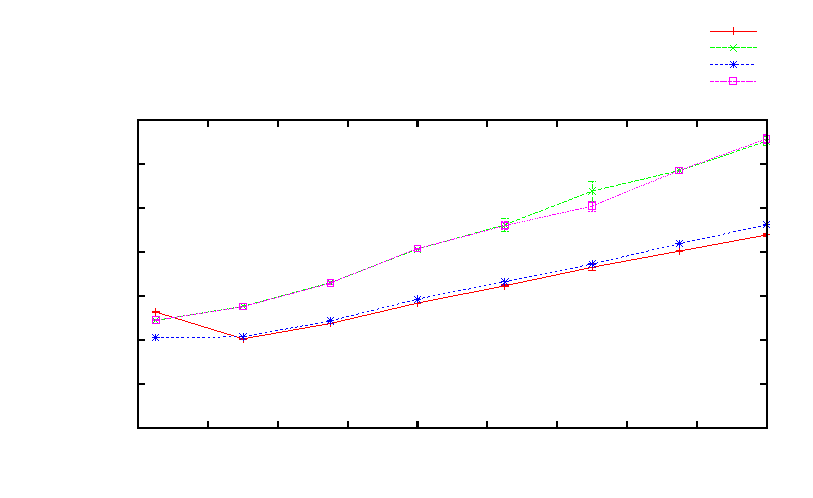
\includegraphics{PrecomputedRankBlockSize_Select_L1CacheMiss}}%
    \gplfronttext
  \end{picture}%
\endgroup

\figureEnd


\figureBegin
\caption{Level 2 Data Cache Misses for Select queries on wavelet trees with precomputed ranks of varying block sizes}
\label{fig:PrecomputedRankBlockSize_Select_L2CacheMiss}
% GNUPLOT: LaTeX picture with Postscript
\begingroup
  \makeatletter
  \providecommand\color[2][]{%
    \GenericError{(gnuplot) \space\space\space\@spaces}{%
      Package color not loaded in conjunction with
      terminal option `colourtext'%
    }{See the gnuplot documentation for explanation.%
    }{Either use 'blacktext' in gnuplot or load the package
      color.sty in LaTeX.}%
    \renewcommand\color[2][]{}%
  }%
  \providecommand\includegraphics[2][]{%
    \GenericError{(gnuplot) \space\space\space\@spaces}{%
      Package graphicx or graphics not loaded%
    }{See the gnuplot documentation for explanation.%
    }{The gnuplot epslatex terminal needs graphicx.sty or graphics.sty.}%
    \renewcommand\includegraphics[2][]{}%
  }%
  \providecommand\rotatebox[2]{#2}%
  \@ifundefined{ifGPcolor}{%
    \newif\ifGPcolor
    \GPcolortrue
  }{}%
  \@ifundefined{ifGPblacktext}{%
    \newif\ifGPblacktext
    \GPblacktexttrue
  }{}%
  % define a \g@addto@macro without @ in the name:
  \let\gplgaddtomacro\g@addto@macro
  % define empty templates for all commands taking text:
  \gdef\gplbacktext{}%
  \gdef\gplfronttext{}%
  \makeatother
  \ifGPblacktext
    % no textcolor at all
    \def\colorrgb#1{}%
    \def\colorgray#1{}%
  \else
    % gray or color?
    \ifGPcolor
      \def\colorrgb#1{\color[rgb]{#1}}%
      \def\colorgray#1{\color[gray]{#1}}%
      \expandafter\def\csname LTw\endcsname{\color{white}}%
      \expandafter\def\csname LTb\endcsname{\color{black}}%
      \expandafter\def\csname LTa\endcsname{\color{black}}%
      \expandafter\def\csname LT0\endcsname{\color[rgb]{1,0,0}}%
      \expandafter\def\csname LT1\endcsname{\color[rgb]{0,1,0}}%
      \expandafter\def\csname LT2\endcsname{\color[rgb]{0,0,1}}%
      \expandafter\def\csname LT3\endcsname{\color[rgb]{1,0,1}}%
      \expandafter\def\csname LT4\endcsname{\color[rgb]{0,1,1}}%
      \expandafter\def\csname LT5\endcsname{\color[rgb]{1,1,0}}%
      \expandafter\def\csname LT6\endcsname{\color[rgb]{0,0,0}}%
      \expandafter\def\csname LT7\endcsname{\color[rgb]{1,0.3,0}}%
      \expandafter\def\csname LT8\endcsname{\color[rgb]{0.5,0.5,0.5}}%
    \else
      % gray
      \def\colorrgb#1{\color{black}}%
      \def\colorgray#1{\color[gray]{#1}}%
      \expandafter\def\csname LTw\endcsname{\color{white}}%
      \expandafter\def\csname LTb\endcsname{\color{black}}%
      \expandafter\def\csname LTa\endcsname{\color{black}}%
      \expandafter\def\csname LT0\endcsname{\color{black}}%
      \expandafter\def\csname LT1\endcsname{\color{black}}%
      \expandafter\def\csname LT2\endcsname{\color{black}}%
      \expandafter\def\csname LT3\endcsname{\color{black}}%
      \expandafter\def\csname LT4\endcsname{\color{black}}%
      \expandafter\def\csname LT5\endcsname{\color{black}}%
      \expandafter\def\csname LT6\endcsname{\color{black}}%
      \expandafter\def\csname LT7\endcsname{\color{black}}%
      \expandafter\def\csname LT8\endcsname{\color{black}}%
    \fi
  \fi
  \setlength{\unitlength}{0.0500bp}%
  \begin{picture}(7488.00,4464.00)%
    \gplgaddtomacro\gplbacktext{%
      \csname LTb\endcsname%
      \put(976,512){\makebox(0,0)[r]{\strut{} 0}}%
      \put(976,808){\makebox(0,0)[r]{\strut{} 20000}}%
      \put(976,1104){\makebox(0,0)[r]{\strut{} 40000}}%
      \put(976,1400){\makebox(0,0)[r]{\strut{} 60000}}%
      \put(976,1696){\makebox(0,0)[r]{\strut{} 80000}}%
      \put(976,1992){\makebox(0,0)[r]{\strut{} 100000}}%
      \put(976,2287){\makebox(0,0)[r]{\strut{} 120000}}%
      \put(976,2583){\makebox(0,0)[r]{\strut{} 140000}}%
      \put(976,2879){\makebox(0,0)[r]{\strut{} 160000}}%
      \put(976,3175){\makebox(0,0)[r]{\strut{} 180000}}%
      \put(976,3471){\makebox(0,0)[r]{\strut{} 200000}}%
      \put(1072,352){\makebox(0,0){\strut{} 0.2}}%
      \put(1753,352){\makebox(0,0){\strut{} 0.4}}%
      \put(2434,352){\makebox(0,0){\strut{} 0.6}}%
      \put(3114,352){\makebox(0,0){\strut{} 0.8}}%
      \put(3795,352){\makebox(0,0){\strut{} 1}}%
      \put(4476,352){\makebox(0,0){\strut{} 1.2}}%
      \put(5157,352){\makebox(0,0){\strut{} 1.4}}%
      \put(5837,352){\makebox(0,0){\strut{} 1.6}}%
      \put(6518,352){\makebox(0,0){\strut{} 1.8}}%
      \put(7199,352){\makebox(0,0){\strut{} 2}}%
      \put(128,1991){\rotatebox{-270}{\makebox(0,0){\strut{}Cache Misses}}}%
      \put(4135,112){\makebox(0,0){\strut{}Block Size (number of pages)}}%
    }%
    \gplgaddtomacro\gplfronttext{%
      \csname LTb\endcsname%
      \put(6560,4321){\makebox(0,0)[r]{\strut{}NaivePrecomputed, $mr\hat{\sigma}=$ 3.73 $avg\hat{\sigma}=$ 1.26}}%
      \csname LTb\endcsname%
      \put(6560,4161){\makebox(0,0)[r]{\strut{}PreallocatedPrecomputed, $mr\hat{\sigma}=$ 2.73 $avg\hat{\sigma}=$ 0.84}}%
      \csname LTb\endcsname%
      \put(6560,4001){\makebox(0,0)[r]{\strut{}UnalignedNaivePrecomputed, $mr\hat{\sigma}=$ 1.68 $avg\hat{\sigma}=$ 0.95}}%
      \csname LTb\endcsname%
      \put(6560,3841){\makebox(0,0)[r]{\strut{}UnalignedPreallocatedPrecomputed, $mr\hat{\sigma}=$ 1.69 $avg\hat{\sigma}=$ 1.09}}%
    }%
    \gplbacktext
    \put(0,0){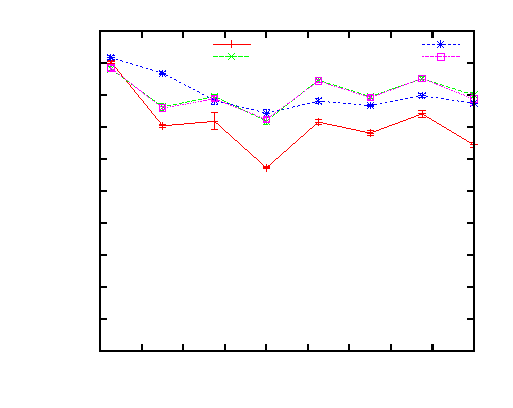
\includegraphics{PrecomputedRankBlockSize_Select_L2CacheMiss}}%
    \gplfronttext
  \end{picture}%
\endgroup

\figureEnd


\figureBegin
\caption{Level 2 Data Cache Miss Rate for Select queries on wavelet trees with precomputed ranks of varying block sizes}
\label{fig:PrecomputedRankBlockSize_Select_L2CacheMissRate}
% GNUPLOT: LaTeX picture with Postscript
\begingroup
  \makeatletter
  \providecommand\color[2][]{%
    \GenericError{(gnuplot) \space\space\space\@spaces}{%
      Package color not loaded in conjunction with
      terminal option `colourtext'%
    }{See the gnuplot documentation for explanation.%
    }{Either use 'blacktext' in gnuplot or load the package
      color.sty in LaTeX.}%
    \renewcommand\color[2][]{}%
  }%
  \providecommand\includegraphics[2][]{%
    \GenericError{(gnuplot) \space\space\space\@spaces}{%
      Package graphicx or graphics not loaded%
    }{See the gnuplot documentation for explanation.%
    }{The gnuplot epslatex terminal needs graphicx.sty or graphics.sty.}%
    \renewcommand\includegraphics[2][]{}%
  }%
  \providecommand\rotatebox[2]{#2}%
  \@ifundefined{ifGPcolor}{%
    \newif\ifGPcolor
    \GPcolortrue
  }{}%
  \@ifundefined{ifGPblacktext}{%
    \newif\ifGPblacktext
    \GPblacktexttrue
  }{}%
  % define a \g@addto@macro without @ in the name:
  \let\gplgaddtomacro\g@addto@macro
  % define empty templates for all commands taking text:
  \gdef\gplbacktext{}%
  \gdef\gplfronttext{}%
  \makeatother
  \ifGPblacktext
    % no textcolor at all
    \def\colorrgb#1{}%
    \def\colorgray#1{}%
  \else
    % gray or color?
    \ifGPcolor
      \def\colorrgb#1{\color[rgb]{#1}}%
      \def\colorgray#1{\color[gray]{#1}}%
      \expandafter\def\csname LTw\endcsname{\color{white}}%
      \expandafter\def\csname LTb\endcsname{\color{black}}%
      \expandafter\def\csname LTa\endcsname{\color{black}}%
      \expandafter\def\csname LT0\endcsname{\color[rgb]{1,0,0}}%
      \expandafter\def\csname LT1\endcsname{\color[rgb]{0,1,0}}%
      \expandafter\def\csname LT2\endcsname{\color[rgb]{0,0,1}}%
      \expandafter\def\csname LT3\endcsname{\color[rgb]{1,0,1}}%
      \expandafter\def\csname LT4\endcsname{\color[rgb]{0,1,1}}%
      \expandafter\def\csname LT5\endcsname{\color[rgb]{1,1,0}}%
      \expandafter\def\csname LT6\endcsname{\color[rgb]{0,0,0}}%
      \expandafter\def\csname LT7\endcsname{\color[rgb]{1,0.3,0}}%
      \expandafter\def\csname LT8\endcsname{\color[rgb]{0.5,0.5,0.5}}%
    \else
      % gray
      \def\colorrgb#1{\color{black}}%
      \def\colorgray#1{\color[gray]{#1}}%
      \expandafter\def\csname LTw\endcsname{\color{white}}%
      \expandafter\def\csname LTb\endcsname{\color{black}}%
      \expandafter\def\csname LTa\endcsname{\color{black}}%
      \expandafter\def\csname LT0\endcsname{\color{black}}%
      \expandafter\def\csname LT1\endcsname{\color{black}}%
      \expandafter\def\csname LT2\endcsname{\color{black}}%
      \expandafter\def\csname LT3\endcsname{\color{black}}%
      \expandafter\def\csname LT4\endcsname{\color{black}}%
      \expandafter\def\csname LT5\endcsname{\color{black}}%
      \expandafter\def\csname LT6\endcsname{\color{black}}%
      \expandafter\def\csname LT7\endcsname{\color{black}}%
      \expandafter\def\csname LT8\endcsname{\color{black}}%
    \fi
  \fi
  \setlength{\unitlength}{0.0500bp}%
  \begin{picture}(7488.00,4464.00)%
    \gplgaddtomacro\gplbacktext{%
      \csname LTb\endcsname%
      \put(1078,704){\makebox(0,0)[r]{\strut{} 0}}%
      \put(1078,1078){\makebox(0,0)[r]{\strut{} 0.05}}%
      \put(1078,1451){\makebox(0,0)[r]{\strut{} 0.1}}%
      \put(1078,1825){\makebox(0,0)[r]{\strut{} 0.15}}%
      \put(1078,2198){\makebox(0,0)[r]{\strut{} 0.2}}%
      \put(1078,2572){\makebox(0,0)[r]{\strut{} 0.25}}%
      \put(1078,2945){\makebox(0,0)[r]{\strut{} 0.3}}%
      \put(1078,3319){\makebox(0,0)[r]{\strut{} 0.35}}%
      \put(1210,484){\makebox(0,0){\strut{} 0}}%
      \put(1945,484){\makebox(0,0){\strut{} 0.5}}%
      \put(2680,484){\makebox(0,0){\strut{} 1}}%
      \put(3415,484){\makebox(0,0){\strut{} 1.5}}%
      \put(4151,484){\makebox(0,0){\strut{} 2}}%
      \put(4886,484){\makebox(0,0){\strut{} 2.5}}%
      \put(5621,484){\makebox(0,0){\strut{} 3}}%
      \put(6356,484){\makebox(0,0){\strut{} 3.5}}%
      \put(7091,484){\makebox(0,0){\strut{} 4}}%
      \put(176,2011){\rotatebox{-270}{\makebox(0,0){\strut{}Cache Miss Rate}}}%
      \put(4150,154){\makebox(0,0){\strut{}Block Size (number of pages)}}%
    }%
    \gplgaddtomacro\gplfronttext{%
      \csname LTb\endcsname%
      \put(6468,4291){\makebox(0,0)[r]{\strut{}NaivePrecomputed, $mr\hat{\sigma}=$ 0.65 $avg\hat{\sigma}=$ 0.65}}%
      \csname LTb\endcsname%
      \put(6468,4071){\makebox(0,0)[r]{\strut{}PreallocatedPrecomputed, $mr\hat{\sigma}=$ 0.46 $avg\hat{\sigma}=$ 0.46}}%
      \csname LTb\endcsname%
      \put(6468,3851){\makebox(0,0)[r]{\strut{}UnalignedNaivePrecomputed, $mr\hat{\sigma}=$ 0.63 $avg\hat{\sigma}=$ 0.63}}%
    }%
    \gplbacktext
    \put(0,0){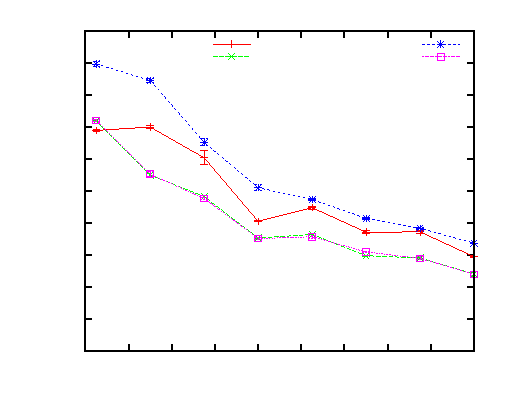
\includegraphics{PrecomputedRankBlockSize_Select_L2CacheMissRate}}%
    \gplfronttext
  \end{picture}%
\endgroup

\figureEnd


\figureBegin
\caption{Level 3 Total Cache Misses for Select queries on wavelet trees with precomputed ranks of varying block sizes}
\label{fig:PrecomputedRankBlockSize_Select_L3CacheMiss}
% GNUPLOT: LaTeX picture with Postscript
\begingroup
  \makeatletter
  \providecommand\color[2][]{%
    \GenericError{(gnuplot) \space\space\space\@spaces}{%
      Package color not loaded in conjunction with
      terminal option `colourtext'%
    }{See the gnuplot documentation for explanation.%
    }{Either use 'blacktext' in gnuplot or load the package
      color.sty in LaTeX.}%
    \renewcommand\color[2][]{}%
  }%
  \providecommand\includegraphics[2][]{%
    \GenericError{(gnuplot) \space\space\space\@spaces}{%
      Package graphicx or graphics not loaded%
    }{See the gnuplot documentation for explanation.%
    }{The gnuplot epslatex terminal needs graphicx.sty or graphics.sty.}%
    \renewcommand\includegraphics[2][]{}%
  }%
  \providecommand\rotatebox[2]{#2}%
  \@ifundefined{ifGPcolor}{%
    \newif\ifGPcolor
    \GPcolortrue
  }{}%
  \@ifundefined{ifGPblacktext}{%
    \newif\ifGPblacktext
    \GPblacktexttrue
  }{}%
  % define a \g@addto@macro without @ in the name:
  \let\gplgaddtomacro\g@addto@macro
  % define empty templates for all commands taking text:
  \gdef\gplbacktext{}%
  \gdef\gplfronttext{}%
  \makeatother
  \ifGPblacktext
    % no textcolor at all
    \def\colorrgb#1{}%
    \def\colorgray#1{}%
  \else
    % gray or color?
    \ifGPcolor
      \def\colorrgb#1{\color[rgb]{#1}}%
      \def\colorgray#1{\color[gray]{#1}}%
      \expandafter\def\csname LTw\endcsname{\color{white}}%
      \expandafter\def\csname LTb\endcsname{\color{black}}%
      \expandafter\def\csname LTa\endcsname{\color{black}}%
      \expandafter\def\csname LT0\endcsname{\color[rgb]{1,0,0}}%
      \expandafter\def\csname LT1\endcsname{\color[rgb]{0,1,0}}%
      \expandafter\def\csname LT2\endcsname{\color[rgb]{0,0,1}}%
      \expandafter\def\csname LT3\endcsname{\color[rgb]{1,0,1}}%
      \expandafter\def\csname LT4\endcsname{\color[rgb]{0,1,1}}%
      \expandafter\def\csname LT5\endcsname{\color[rgb]{1,1,0}}%
      \expandafter\def\csname LT6\endcsname{\color[rgb]{0,0,0}}%
      \expandafter\def\csname LT7\endcsname{\color[rgb]{1,0.3,0}}%
      \expandafter\def\csname LT8\endcsname{\color[rgb]{0.5,0.5,0.5}}%
    \else
      % gray
      \def\colorrgb#1{\color{black}}%
      \def\colorgray#1{\color[gray]{#1}}%
      \expandafter\def\csname LTw\endcsname{\color{white}}%
      \expandafter\def\csname LTb\endcsname{\color{black}}%
      \expandafter\def\csname LTa\endcsname{\color{black}}%
      \expandafter\def\csname LT0\endcsname{\color{black}}%
      \expandafter\def\csname LT1\endcsname{\color{black}}%
      \expandafter\def\csname LT2\endcsname{\color{black}}%
      \expandafter\def\csname LT3\endcsname{\color{black}}%
      \expandafter\def\csname LT4\endcsname{\color{black}}%
      \expandafter\def\csname LT5\endcsname{\color{black}}%
      \expandafter\def\csname LT6\endcsname{\color{black}}%
      \expandafter\def\csname LT7\endcsname{\color{black}}%
      \expandafter\def\csname LT8\endcsname{\color{black}}%
    \fi
  \fi
  \setlength{\unitlength}{0.0500bp}%
  \begin{picture}(7488.00,4464.00)%
    \gplgaddtomacro\gplbacktext{%
      \csname LTb\endcsname%
      \put(1342,704){\makebox(0,0)[r]{\strut{} 0}}%
      \put(1342,995){\makebox(0,0)[r]{\strut{} 20000}}%
      \put(1342,1285){\makebox(0,0)[r]{\strut{} 40000}}%
      \put(1342,1576){\makebox(0,0)[r]{\strut{} 60000}}%
      \put(1342,1866){\makebox(0,0)[r]{\strut{} 80000}}%
      \put(1342,2157){\makebox(0,0)[r]{\strut{} 100000}}%
      \put(1342,2447){\makebox(0,0)[r]{\strut{} 120000}}%
      \put(1342,2738){\makebox(0,0)[r]{\strut{} 140000}}%
      \put(1342,3028){\makebox(0,0)[r]{\strut{} 160000}}%
      \put(1342,3319){\makebox(0,0)[r]{\strut{} 180000}}%
      \put(1474,484){\makebox(0,0){\strut{} 0.2}}%
      \put(2098,484){\makebox(0,0){\strut{} 0.4}}%
      \put(2722,484){\makebox(0,0){\strut{} 0.6}}%
      \put(3346,484){\makebox(0,0){\strut{} 0.8}}%
      \put(3970,484){\makebox(0,0){\strut{} 1}}%
      \put(4595,484){\makebox(0,0){\strut{} 1.2}}%
      \put(5219,484){\makebox(0,0){\strut{} 1.4}}%
      \put(5843,484){\makebox(0,0){\strut{} 1.6}}%
      \put(6467,484){\makebox(0,0){\strut{} 1.8}}%
      \put(7091,484){\makebox(0,0){\strut{} 2}}%
      \put(176,2011){\rotatebox{-270}{\makebox(0,0){\strut{}Cache Misses}}}%
      \put(4282,154){\makebox(0,0){\strut{}Block Size (number of pages)}}%
    }%
    \gplgaddtomacro\gplfronttext{%
      \csname LTb\endcsname%
      \put(6468,4291){\makebox(0,0)[r]{\strut{}NaivePrecomputed, $mr\hat{\sigma}=$ 2.31 $avg\hat{\sigma}=$ 1.17}}%
      \csname LTb\endcsname%
      \put(6468,4071){\makebox(0,0)[r]{\strut{}PreallocatedPrecomputed, $mr\hat{\sigma}=$ 1.26 $avg\hat{\sigma}=$ 0.79}}%
      \csname LTb\endcsname%
      \put(6468,3851){\makebox(0,0)[r]{\strut{}UnalignedNaivePrecomputed, $mr\hat{\sigma}=$ 1.56 $avg\hat{\sigma}=$ 1.08}}%
    }%
    \gplbacktext
    \put(0,0){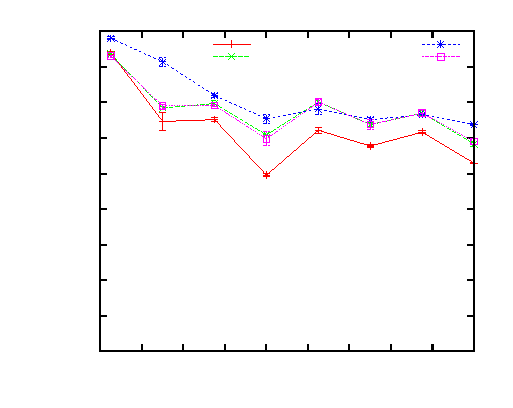
\includegraphics{PrecomputedRankBlockSize_Select_L3CacheMiss}}%
    \gplfronttext
  \end{picture}%
\endgroup

\figureEnd


\subsubsection{Memory Usage of Concatenated vs. Individual Bitmaps}

\figureBegin
\caption{Difference in Memory Usage of wavelet trees with precomputed ranks of varying block size. Notice the y-axis not starting at 0. Limited to 2 times page size because of use of \texttt{ushort}}
\label{fig:PrecomputedRankBlockSize_MemoryUsage}
% GNUPLOT: LaTeX picture with Postscript
\begingroup
  \makeatletter
  \providecommand\color[2][]{%
    \GenericError{(gnuplot) \space\space\space\@spaces}{%
      Package color not loaded in conjunction with
      terminal option `colourtext'%
    }{See the gnuplot documentation for explanation.%
    }{Either use 'blacktext' in gnuplot or load the package
      color.sty in LaTeX.}%
    \renewcommand\color[2][]{}%
  }%
  \providecommand\includegraphics[2][]{%
    \GenericError{(gnuplot) \space\space\space\@spaces}{%
      Package graphicx or graphics not loaded%
    }{See the gnuplot documentation for explanation.%
    }{The gnuplot epslatex terminal needs graphicx.sty or graphics.sty.}%
    \renewcommand\includegraphics[2][]{}%
  }%
  \providecommand\rotatebox[2]{#2}%
  \@ifundefined{ifGPcolor}{%
    \newif\ifGPcolor
    \GPcolortrue
  }{}%
  \@ifundefined{ifGPblacktext}{%
    \newif\ifGPblacktext
    \GPblacktexttrue
  }{}%
  % define a \g@addto@macro without @ in the name:
  \let\gplgaddtomacro\g@addto@macro
  % define empty templates for all commands taking text:
  \gdef\gplbacktext{}%
  \gdef\gplfronttext{}%
  \makeatother
  \ifGPblacktext
    % no textcolor at all
    \def\colorrgb#1{}%
    \def\colorgray#1{}%
  \else
    % gray or color?
    \ifGPcolor
      \def\colorrgb#1{\color[rgb]{#1}}%
      \def\colorgray#1{\color[gray]{#1}}%
      \expandafter\def\csname LTw\endcsname{\color{white}}%
      \expandafter\def\csname LTb\endcsname{\color{black}}%
      \expandafter\def\csname LTa\endcsname{\color{black}}%
      \expandafter\def\csname LT0\endcsname{\color[rgb]{1,0,0}}%
      \expandafter\def\csname LT1\endcsname{\color[rgb]{0,1,0}}%
      \expandafter\def\csname LT2\endcsname{\color[rgb]{0,0,1}}%
      \expandafter\def\csname LT3\endcsname{\color[rgb]{1,0,1}}%
      \expandafter\def\csname LT4\endcsname{\color[rgb]{0,1,1}}%
      \expandafter\def\csname LT5\endcsname{\color[rgb]{1,1,0}}%
      \expandafter\def\csname LT6\endcsname{\color[rgb]{0,0,0}}%
      \expandafter\def\csname LT7\endcsname{\color[rgb]{1,0.3,0}}%
      \expandafter\def\csname LT8\endcsname{\color[rgb]{0.5,0.5,0.5}}%
    \else
      % gray
      \def\colorrgb#1{\color{black}}%
      \def\colorgray#1{\color[gray]{#1}}%
      \expandafter\def\csname LTw\endcsname{\color{white}}%
      \expandafter\def\csname LTb\endcsname{\color{black}}%
      \expandafter\def\csname LTa\endcsname{\color{black}}%
      \expandafter\def\csname LT0\endcsname{\color{black}}%
      \expandafter\def\csname LT1\endcsname{\color{black}}%
      \expandafter\def\csname LT2\endcsname{\color{black}}%
      \expandafter\def\csname LT3\endcsname{\color{black}}%
      \expandafter\def\csname LT4\endcsname{\color{black}}%
      \expandafter\def\csname LT5\endcsname{\color{black}}%
      \expandafter\def\csname LT6\endcsname{\color{black}}%
      \expandafter\def\csname LT7\endcsname{\color{black}}%
      \expandafter\def\csname LT8\endcsname{\color{black}}%
    \fi
  \fi
  \setlength{\unitlength}{0.0500bp}%
  \begin{picture}(7488.00,4464.00)%
    \gplgaddtomacro\gplbacktext{%
      \csname LTb\endcsname%
      \put(1342,704){\makebox(0,0)[r]{\strut{} 820000}}%
      \put(1342,948){\makebox(0,0)[r]{\strut{} 830000}}%
      \put(1342,1193){\makebox(0,0)[r]{\strut{} 840000}}%
      \put(1342,1437){\makebox(0,0)[r]{\strut{} 850000}}%
      \put(1342,1682){\makebox(0,0)[r]{\strut{} 860000}}%
      \put(1342,1926){\makebox(0,0)[r]{\strut{} 870000}}%
      \put(1342,2170){\makebox(0,0)[r]{\strut{} 880000}}%
      \put(1342,2415){\makebox(0,0)[r]{\strut{} 890000}}%
      \put(1342,2659){\makebox(0,0)[r]{\strut{} 900000}}%
      \put(1474,484){\makebox(0,0){\strut{} 0}}%
      \put(2036,484){\makebox(0,0){\strut{} 20}}%
      \put(2597,484){\makebox(0,0){\strut{} 40}}%
      \put(3159,484){\makebox(0,0){\strut{} 60}}%
      \put(3721,484){\makebox(0,0){\strut{} 80}}%
      \put(4283,484){\makebox(0,0){\strut{} 100}}%
      \put(4844,484){\makebox(0,0){\strut{} 120}}%
      \put(5406,484){\makebox(0,0){\strut{} 140}}%
      \put(5968,484){\makebox(0,0){\strut{} 160}}%
      \put(6529,484){\makebox(0,0){\strut{} 180}}%
      \put(7091,484){\makebox(0,0){\strut{} 200}}%
      \put(176,1681){\rotatebox{-270}{\makebox(0,0){\strut{}Memory Usage}}}%
      \put(4282,154){\makebox(0,0){\strut{}Block Size  (x1000 bits)}}%
    }%
    \gplgaddtomacro\gplfronttext{%
      \csname LTb\endcsname%
      \put(6236,4181){\makebox(0,0)[r]{\strut{}NaivePrecomputed, $mr\hat{\sigma}=$1.30 $avg\hat{\sigma}=$0.63}}%
      \csname LTb\endcsname%
      \put(6236,3741){\makebox(0,0)[r]{\strut{}PreallocatedPrecomputed, $mr\hat{\sigma}=$11.79 $avg\hat{\sigma}=$3.33}}%
      \csname LTb\endcsname%
      \put(6236,3301){\makebox(0,0)[r]{\strut{}UnalignedNaivePrecomputed, $mr\hat{\sigma}=$1.88 $avg\hat{\sigma}=$0.69}}%
    }%
    \gplbacktext
    \put(0,0){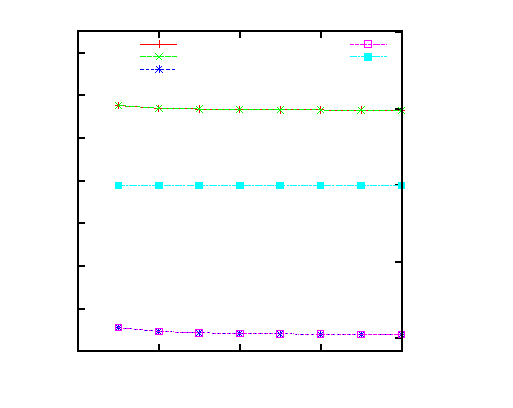
\includegraphics{PrecomputedRankBlockSize_MemoryUsage}}%
    \gplfronttext
  \end{picture}%
\endgroup

\figureEnd